\section{Results}\label{chap:results}



%=====================
% Dice Two
%=====================

\subsection{Accuracy of the Potential in Dependance of the Number of Mass Bins}


Fig. \ref{fig:dice-two-binning} shows potentials computed with different numbers of mass bins, ranging from 10 to 10'000, and different binning distances (linear or logarithmic).
The potentials are computed for the subhalo of the \dt-dataset.
The results of 10'000 bins were taken as a reference point, which contain $\sim 5$ particles per bin on average.
Figure \ref{fig:dice-two-binning-analysis} shows the standard deviation $\sigma_N$ and the maximal deviation $D_{max,N}$ of the potential obtained with $N$ bins computed with
%Table \ref{tab:dice-two-binning-analysis} shows the total deviation $D_{tot,N}$ and the maximal deviation $D_{max,N}$ of the potential obtained with $N$ bins computed with
%
\begin{align}
	\sigma_N &= \left[ \frac{1}{N} \sum\limits_{i} \left( \frac{\phi(r_i)_N }{\phi(r_{i})_{10'000}} -1 \right)^2 \ \right] ^{\frac{1}{2}} \label{eq:Dtot} \\
	D_{max,N} &= \max \limits_{i} \left\{ \ \left | \frac{\phi(r_i)_N }{\phi(r_{i})_{10'000}} - 1 \right | \ \right\} \label{eq:Dmax}
\end{align}
%
where $r_{max}$ is the distance of the particle furthest away from the centre of mass ($r_{CoM}=0$ ). 
%$\phi(r_{max})$ is the potential at that distance, which is identical in all cases and for this reason used as a unit for the computation of the deviations.











\begin{figure}[!h]
	\centering
	\fbox{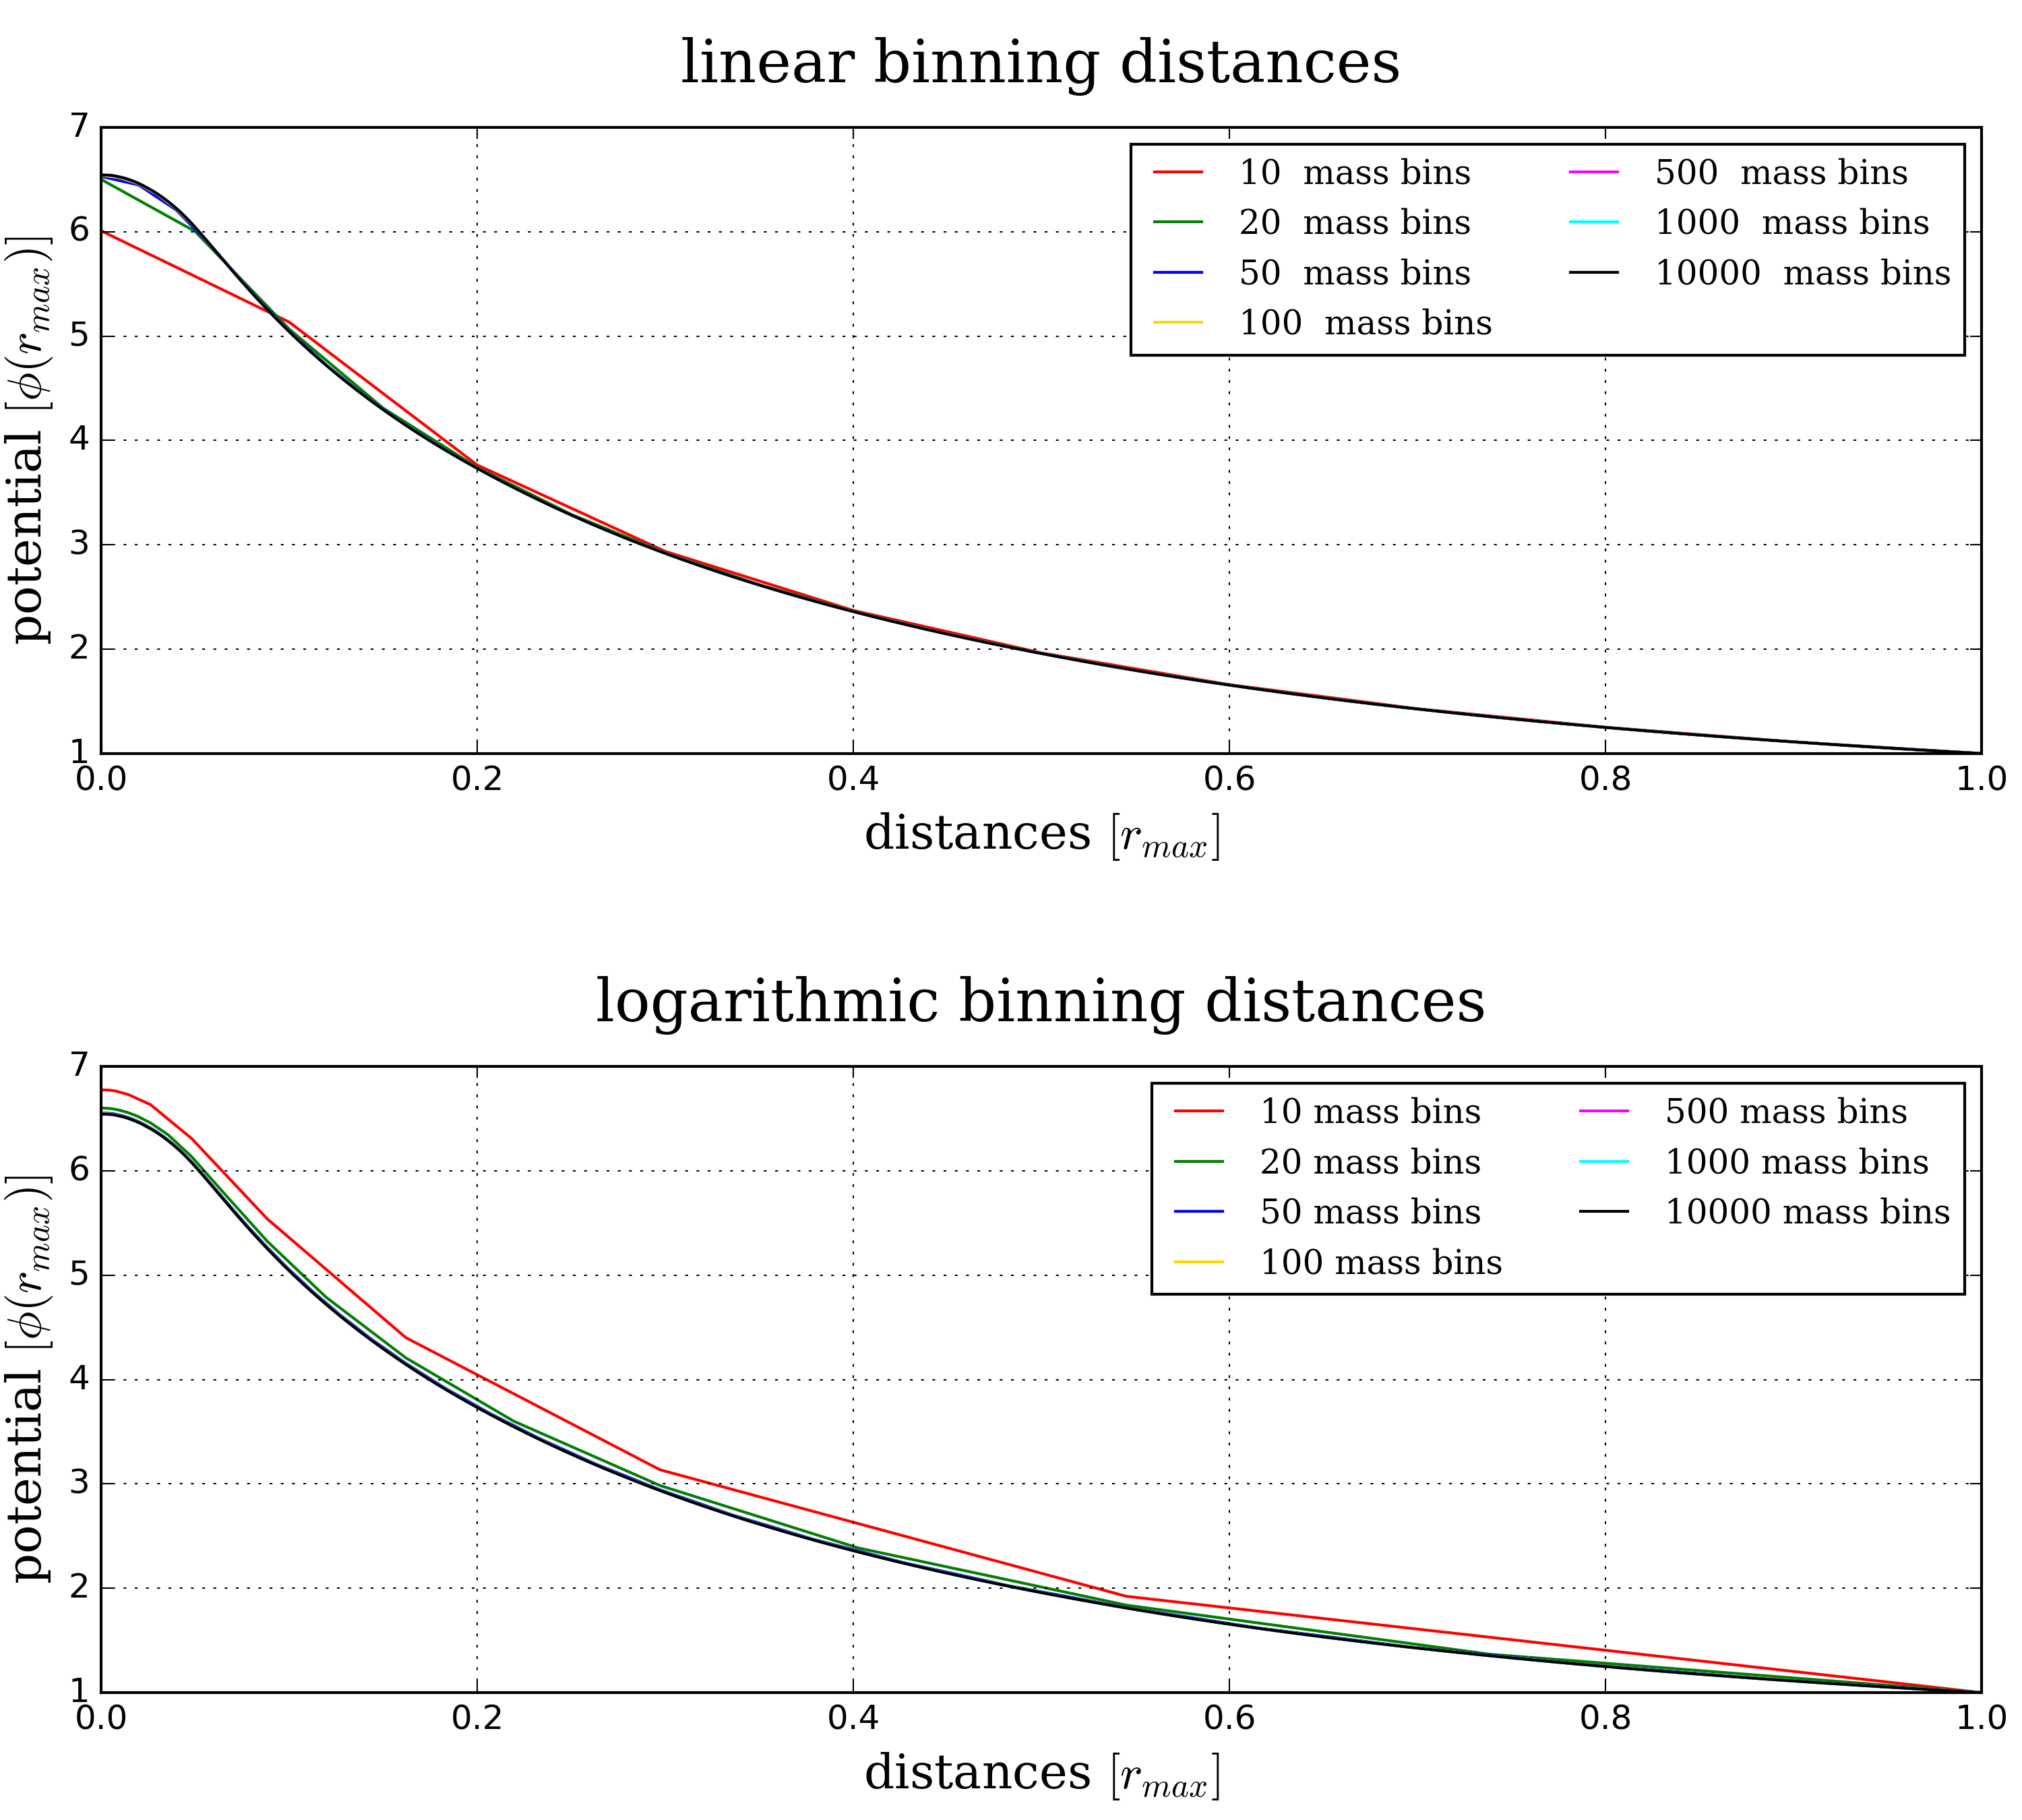
\includegraphics[width=.7\textwidth]{images/dice-two/phi_plot_4220_lin.png}}%
	\caption{
		The potential of the subhalo clump of the \dt-dataset computed with different binning methods and bin numbers.
		$r_{max}$ is the distance of the particle furthest away from the centre of mass, which is set at $r=0$
	}%
	\label{fig:dice-two-binning}
\end{figure}

\begin{figure}[!h]
	\centering
	\fbox{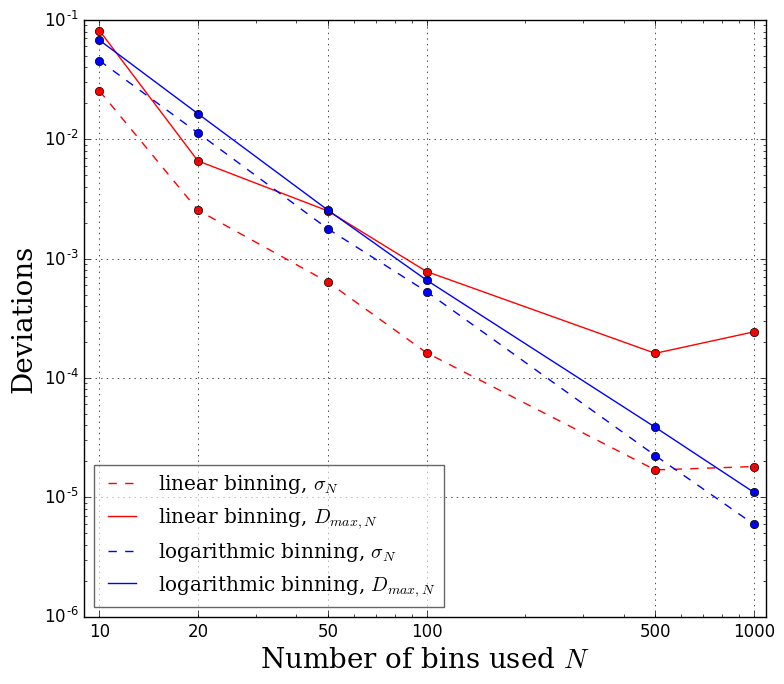
\includegraphics[width=.5\textwidth, keepaspectratio]{images/dice-two/phi_errors_plot_4220.png}}%
	\caption{ 
		Standard deviation $\sigma_N$ and maximal deviation $D_{max,N}$ of the potential obtained with $N$ bins, computed according to equations \ref{eq:Dtot} and \ref{eq:Dmax}, resp., for the subhalo clump of the \dt-dataset
	}%
	\label{fig:dice-two-binning-analysis}
\end{figure}








For both linear and logarithmic binning distances, the maximal deviation falls well below $1\%$ for 50 mass bins used, and below $0.1 \%$ for 100 mass bins.
Even though the standard deviation of linear binning is smaller for 100 bins, logarithmic bins are used for further tests because the logarithmic binning seems to describe the potential close to the centre of mass better.
This is particularly important when the unbinding includes iterative clump properties determination and considers neighbours, which will be shown in section \ref{chap:unbindings}.

Notably, the potential obtained with 10 bins and logarithmic binning distances seems to be the only one deviating on every point.
This is caused by the way the integral for the potential is computed:
%The computation of the integral is always between two bins.
As the bin widths grow for logarithmic binning distances, the accuracy decreases.
The error for 10 bins and logarithmic binning distances should be the highest of all.
Once the integral of each bin is computed, the integral is then summed up beginning at the outermost bin with respect to the centre of mass, so a large error at the first bin will propagate through every other bin. 





















\subsection{Effect of Iterative Clump Properties Determination}\label{chap:iter}

\begin{table}[!htb]
	\begin{centering}
		\begin{tabular}[t]{|r | l | r | l |}
			\hline
			$\varepsilon$     &       $d_v$ 	& \texttt{niter}  		&	$D_v$	\\
			\hline
			0.5       &        0.3000  	&  		 		2    	&	0.2326  \\
			0.1       &        0.0614  	&           	4    	&	0.0419	\\
			0.01      &        0.0036  	&           	7    	&	0.0024	\\
			0.001     &        0.0010  	&           	8    	&	0.0014  \\       
			0.0001    &        0.0000  	&          		10    	&	0.0009 	\\
			\hline
		\end{tabular}
	\caption{%
			The deviation $D_v$ (eq. \ref{eq:Dv}) from the originally set bulk velocity to the computed bulk velocity for the subhalo of the \dt-dataset in dependence of the convergence limit $\varepsilon$.
			The iterative clump properties determination halts after \texttt{niter} iterations, when the difference $d_v$ of the previously determined bulk velocity to the new bulk velocity, $d_v = \frac{v_{bulk} - v_{bulk,old}}{v_{bulk,old}} < \varepsilon$.
	}
	\label{tab:converging}%
	\end{centering}
\end{table}


For the \dt-dataset, the precise relative velocity of the two clumps is known.
Table \ref{tab:converging} shows the deviation $D_v$ of the computed clump bulk velocity $v_{bulk}$ from the original bulk velocity $v_{orig}$ as set with \dice\ with decreasing converging limits $\varepsilon$.
$D_v$ is computed as follows:
%
\begin{align}
	D_v = \left | 	 \frac{v_{bulk} - v_{orig}}{v_{orig}}				\right | \label{eq:Dv}
\end{align} 
%
The deviation falls below $1\%$ for $\varepsilon = 0.01$, which is why that value will be used for further tests.






















\subsection{Effects of Different Unbinding Methods}\label{chap:unbindings}

Taking neighbouring structures into account and determining clump properties iteratively are attempts to improve the accuracy of the particle unbinding, but can be left out if desired.
In this section, the results of three different unbinding methods on the three previously introduced datasets as well as the results as found by the clump finder without unbinding.
The methods are named as follows:
%
%{\centering
%	\begin{tabular}[c]{l p{13cm}}
%		\simple	&	Simple unbinding without considering neighbour clumps for the potential nor determining clump properties iteratively.\\
%		\neigh	& 	Unbinding considering neighbour clumps for the potential \\%as described in section \ref{chap:neighbours} \\
%		\iter	&	Unbinding considering neighbour clumps for the potential and iterative clump properties determination% as described in section \ref{chap:iter_theory}
%	\end{tabular}
%}
\begin{labeling}{\texttt{neighbours}}
	\renewcommand{\arraystretch}{0.1}
 	\item [\simple]		Simple unbinding without considering neighbour clumps for the potential nor determining clump properties iteratively.
	\item [\neigh]		Unbinding considering neighbour clumps for the potential
	\item [\iter]		Unbinding considering neighbour clumps for the potential and iterative clump properties determination
\end{labeling}

%
All three unbinding methods are executed with 100 mass bins and logarithmic binning distances.
For the \iter\ runs, the convergence limit $\varepsilon$ was set to 0.01.
The results without particle unbinding, which are the results as found by \phew, are also the initial situation on which the unbinding is performed.
They are labelled as ``\phewon''.

Table \ref{tab:unbinding_results} shows the number of particles in clumps for these unbinding methods.
For the \cosmo-dataset, all halo-namegiver and subhalo particles have been summed up respectively, because there were too many clumps ($\sim 19'000$) to represent individually.
Furthermore, the particle distributions for all four runs and all three datasets are shown in figures \ref{fig:dice_two_results}, \ref{fig:dice_sub_results} and \ref{fig:cosmo_results}.
In case of the \cosmo-dataset, only one halo and its substructure are shown instead all of them simultaneously, so the effects of the unbinding methods can be seen better.
%There are three plots for each of the four runs: The first contains all particles, the second only the halo-namegiver clump particles, and the last one only the substructure particles.

\begin{table}[!htb]
	{\footnotesize
	\begin{centering}
		\def\arraystretch{1.2}
		\begin{tabular}[t]{ l | R{2.5cm} |  R{2.5cm} |  R{2.5cm} |  R{2.5cm} |}
			%
			%=======================
			% DICE TWO 
			%=======================
			%
			\cline{2-5}
							& \multicolumn{4}{|c|}{\textbf{\dt-dataset}} \\
			\cline{2-5}
							& \phewon    &  \simple & \neigh  & \iter \\
			\hline
			\hline
			halo-namegiver particles 	&	187606	&	202998	& 233450		&	231905	\\
			subhalo particles 			&	52394	&	37002	&	6550	&	8095	\\
			\hline
			\multicolumn{5}{c}{}\\
			%
			%
			%
			%=======================
			% DICE SUB 
			%=======================
			%
			\cline{2-5}
				& \multicolumn{4}{|c|}{\textbf{\ds-dataset}} \\
			\cline{2-5}
				& \phewon    &  \simple & \neigh  & \iter \\
			\hline
			\hline
			halo-namegiver particles 	&	965485	& 	975038	& 1196614	&	1180544	\\
			subhalo particles 			&	197767	&	221977	&	49647	&	58963	\\
			subsubhalo 1 particles 		&	38734	&	23398	&	4475	&	7280	\\
			subsubhalo 2 particles 		&	26591	&	19590	&	5239	&	6151	\\
			subsubhalo 3 particles 		&	31421	&	19995	&	4023	&	7060	\\
			\hline
			\multicolumn{5}{c}{}\\
			%
			%
			%
			%
			%=======================
			% COSMO 
			%=======================
			%
			\cline{2-5}
				& \multicolumn{4}{|c|}{\textbf{\cosmo-dataset}} \\
			\cline{2-5}
				& \phewon    &  \simple & \neigh  & \iter \\
			\hline
			\hline
			halo-namegiver particles 	&	573832	&	640686	&	746441	&	740616	\\
			subhalo particles 			&	188036	&	121182	&	15427	&	21252	\\
			\hline
			\multicolumn{5}{c}{}\\
			%
			%
		\end{tabular}
	\end{centering}
	} %footnotesize
	\caption{%
		The number of particles in clumps depending on the unbinding method for the \dt-, \ds- and \cosmo-dataset.
	}%
	\label{tab:unbinding_results}%
\end{table}


%The effects of the different unbinding methods can be seen very well in the images and the table.
Comparing the results of \phew\ and the \simple\ unbinding of the \dt-dataset in figure \ref{fig:dice_two_results_a} and of the \cosmo-dataset in figure \ref{fig:cosmo_results_a} shows that the \simple\ method already has a decent contribution to the assignment of particles to the structures.
Looking at the halo-namegiver particles only, one can see that where \phew\ has made clean cuts between the clumps, now particles have been re-introduced, yielding smoother structures.

The results of the \simple\ unbinding for the \ds-dataset in fig. \ref{fig:dice_sub_results_a} and table \ref{tab:unbinding_results} show clearly that most unbound particles from the lowest level substructure, the subsubhalos, have been assigned to the parent clump, not to the halo-namegiver.
Note for example that most substructure particles above the subsubhalo 1 (green) are assigned to the subhalo (pink) after \simple\ unbinding.
The surfaces of the subsubhalos facing away from the subhalo appear much more spherical, which is how they were originally created to be.


In all three figures, the effect of considering neighbours for the potential seems drastic.
But recall that when neighbouring clumps are considered for the potential, the particles that remain after unbinding are exclusively bound to the subhalo they are assigned to.
The substructure clumps have indeed been stripped from most of their particles and only what appears to be ``cores'' close to the centre of mass remain, in agreement with what one would expect considering the argumentation used in context with figures \ref{fig:orbits} and \ref{fig:potentials}. 
%This was to be expected, it is in agreement with figure \ref{fig:orbits} that only particles close to the centre of mass will be bound exclusively to the subhalos.
Two subhalos from the halo of the \cosmo-dataset (figure \ref{fig:cosmo_results}, subhalo 1 and 5, have even been stripped of all their particles, indicating that none of their particles can be considered as exclusively bound to them.



The iterative determination of clump properties seems to find overall more bound particles compared to the \neigh\ runs.
In each of the presented cases the total number of particles in substructure grew.
In case of the \cosmo-dataset, 36 clumps had less bound particles (472 particles in total) after \iter-unbinding, while 187 clumps had more bound particles, 6297 in total.


Unfortunately, iterative clump properties determination couldn't re-introduce any particles to the completely unbound subhalos 1 and 5 of the halo shown in fig. \ref{fig:cosmo_results_b}. 
If all particles are unbound at the first iteration already, no new clump properties can be determined and the situation remains as it is.
If necessary, an attempt to improve on this effect might be to first determine clump properties iteratively for such cases and only after the iteration has finished take neighbouring structures into account.
This feature has not been adapted, as no urgent need for it was seen.
It is perfectly plausible that some substructure as identified by \phew\ could contain no exclusively bound particles. 




%=====================
% Dice Two
%=====================

\begin{subfigures}
	\begin{figure}[!htbp]
		{
		\renewcommand{\arraystretch}{0.1}		
		\centering	
	%	\subfloat[]{
		\begin{tabular}{|p{.5cm} c c|}
			\hline
			&&\\[1em]
			&	\phewon\ 	& \simple \\[1.5em]
			%
			%
			\begin{sideways}{\hspace{3cm} \textbf{All particles}}\end{sideways} \hspace*{-1em}	&		 
			{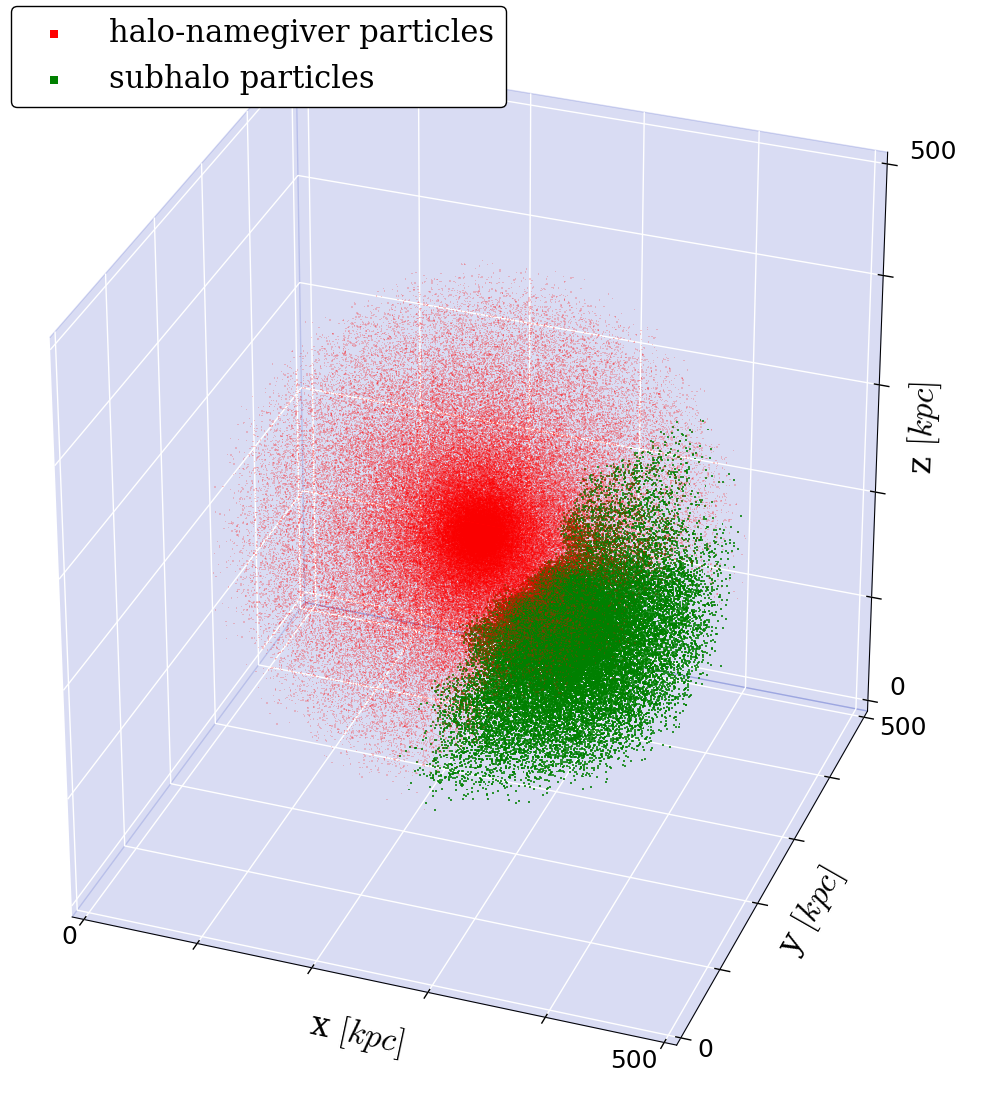
\includegraphics[width = .42\textwidth]{images/dice-two/dice-two-plot-halo1451-phew.png}} \hspace*{-1em} 	& 
			{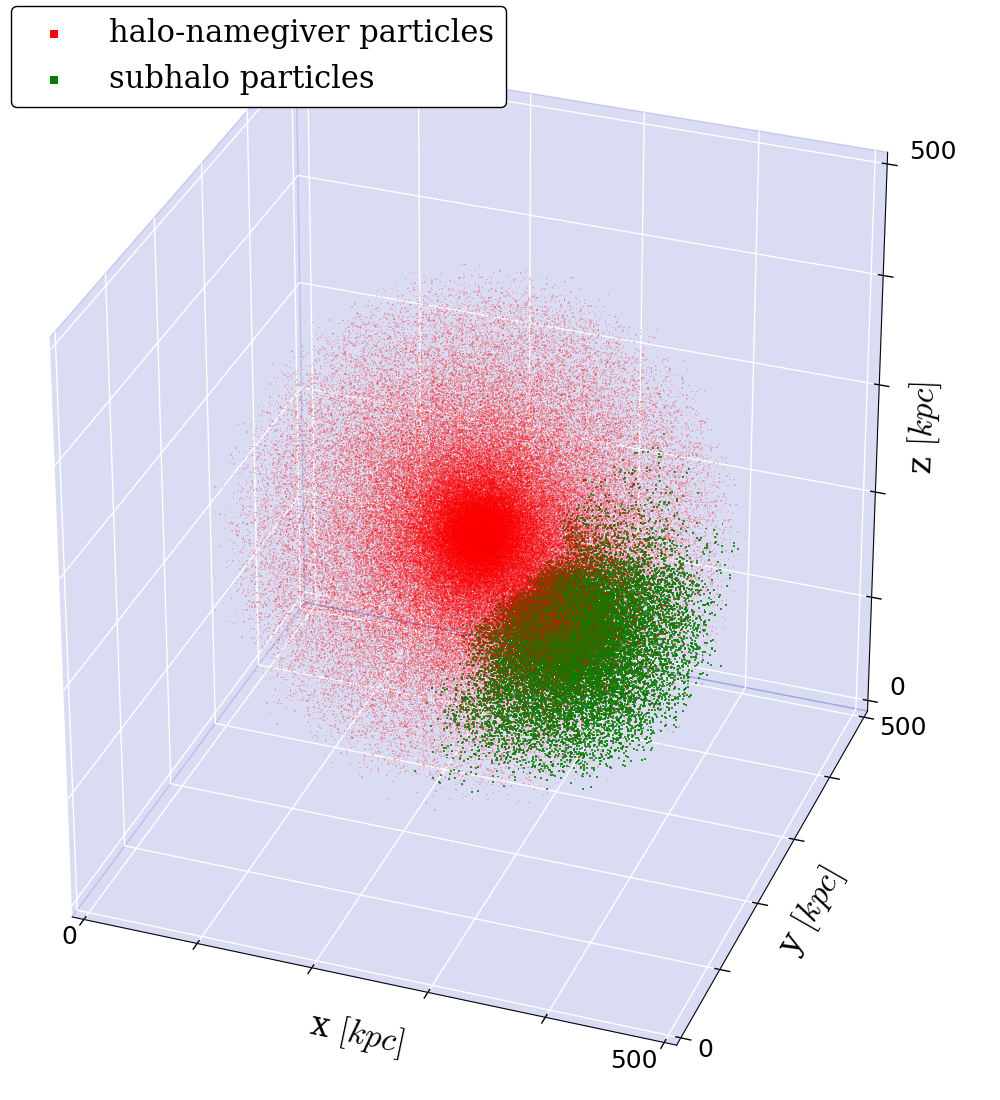
\includegraphics[width = .42\textwidth]{images/dice-two/dice-two-plot-halo1451-nosaddle.png}} \hspace*{-1em}	\\
			%
			%
			\begin{sideways}{ \hspace{.5cm}\textbf{Halo-namegiver particles only} }\end{sideways}	 \hspace*{-1em}			 &			 
			{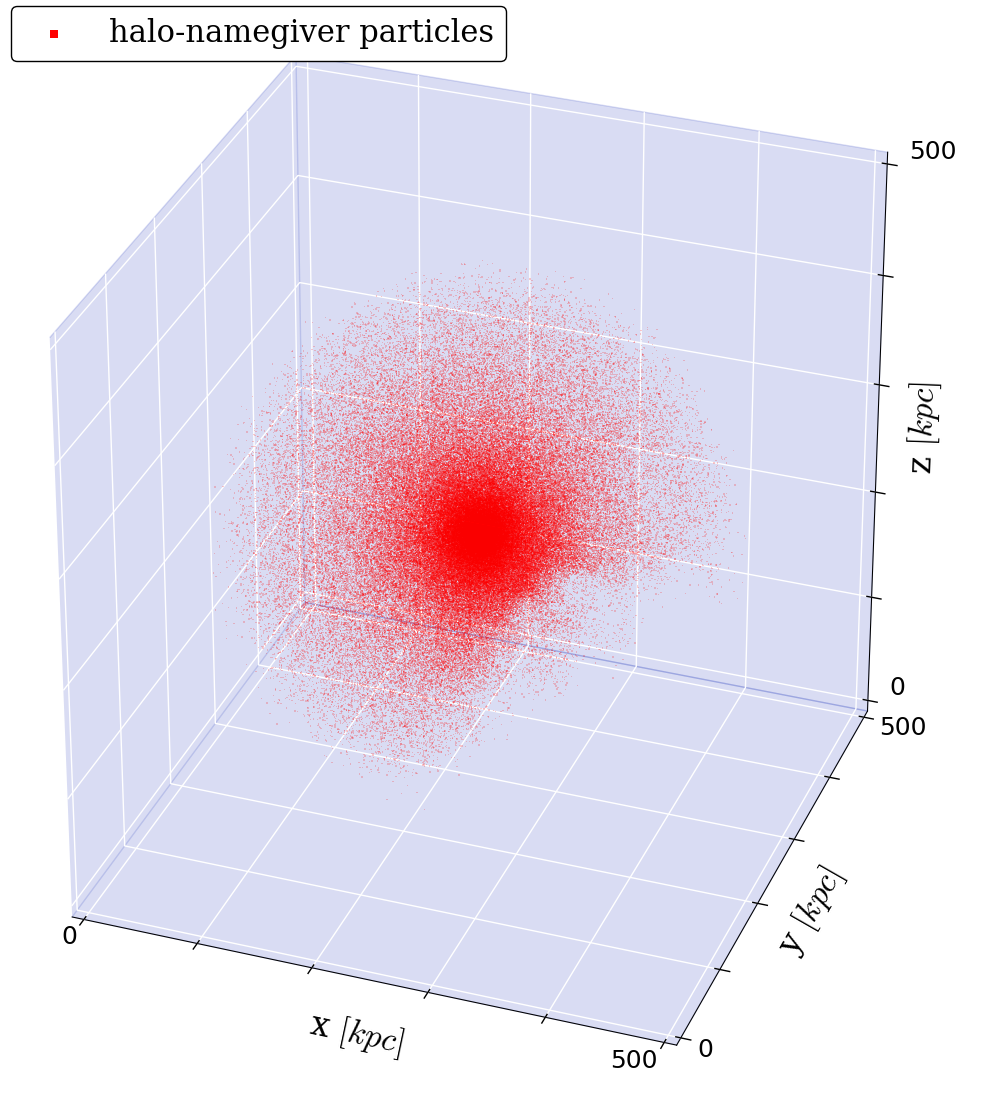
\includegraphics[width = .42\textwidth]{images/dice-two/dice-two-halo-only-phew.png}} \hspace*{-1em} 		&
			{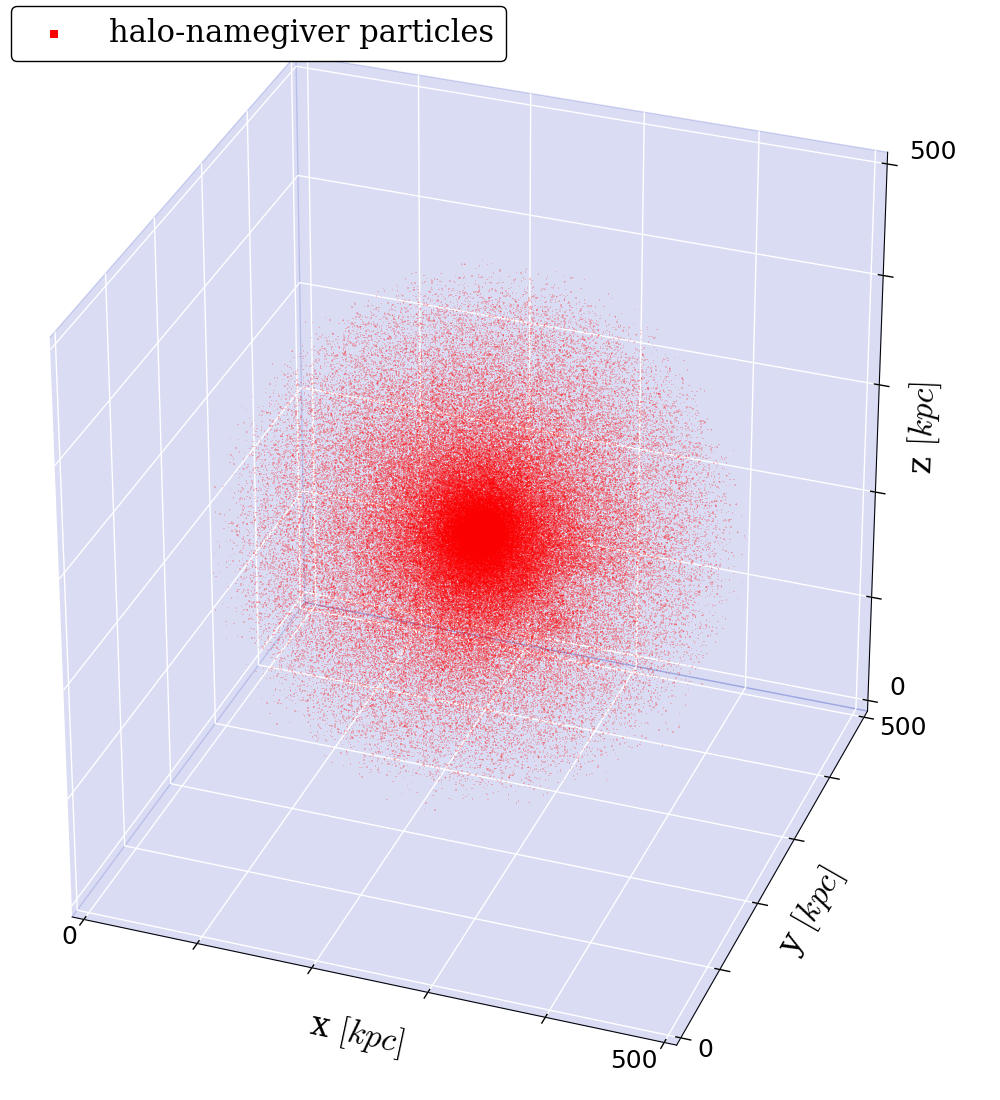
\includegraphics[width = .42\textwidth]{images/dice-two/dice-two-halo-only-nosaddle.png}} \hspace*{-1em}		\\
			%
			%
			\begin{sideways}{ \hspace{2cm}\textbf{Subhalo particles only} }\end{sideways}	 \hspace*{-1em}			 &
			{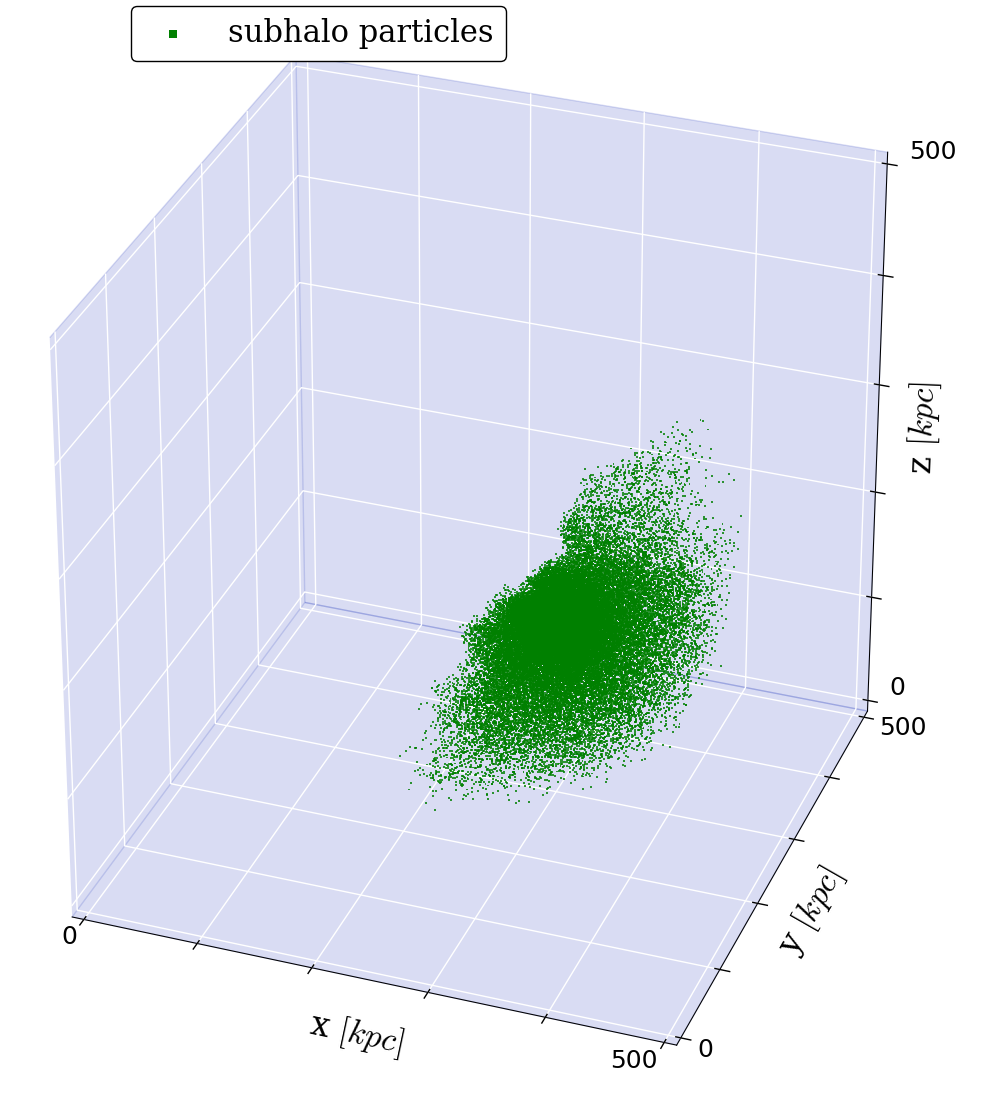
\includegraphics[width = .42\textwidth]{images/dice-two/dice-two-plot-subhalo-phew.png}} &
			{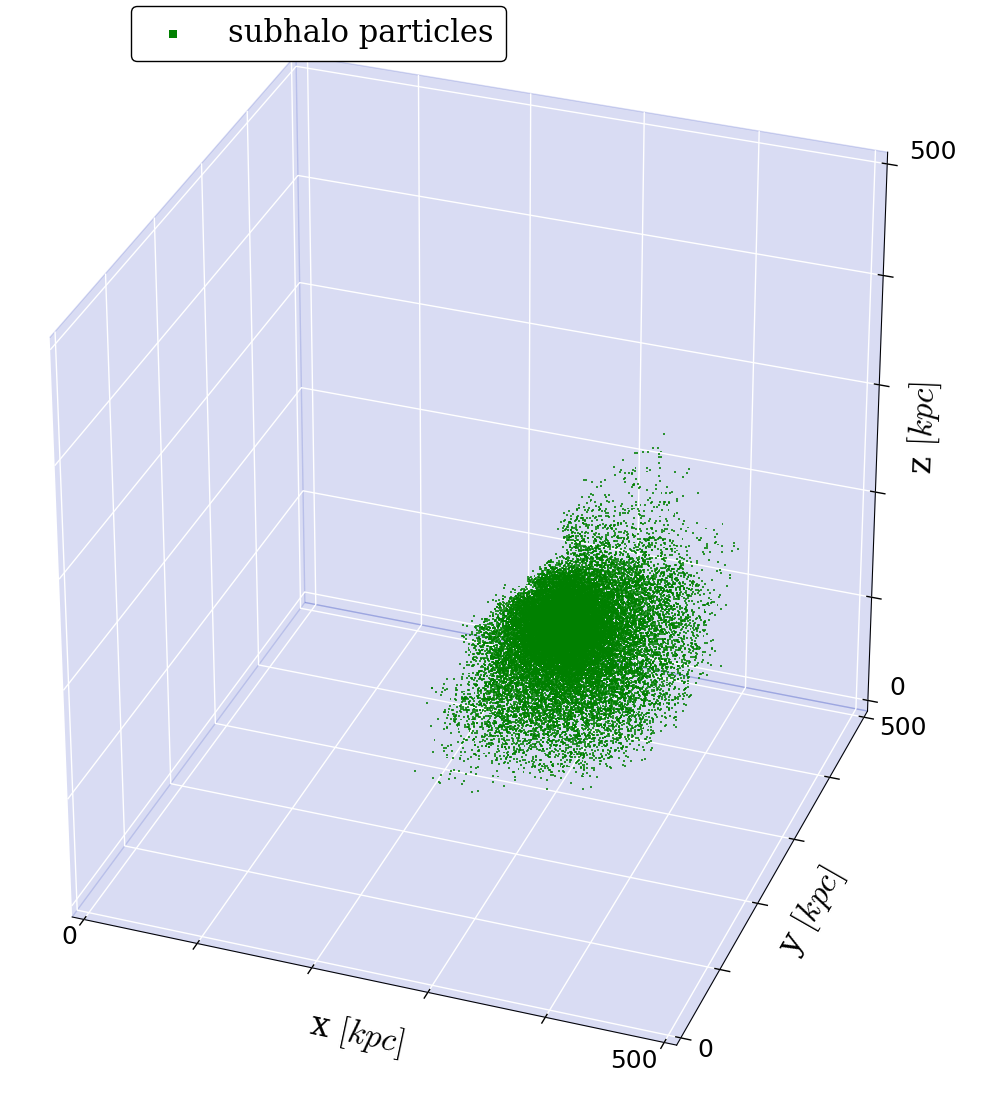
\includegraphics[width = .42\textwidth]{images/dice-two/dice-two-plot-subhalo-nosaddle.png}} \\
			\hline
		\end{tabular}
		\caption{\label{fig:dice_two_results_a}The results of \phewon\ and \simple\ unbinding of the \dt-dataset: All particles, halo-namegiver particles only and subhalo particles only.}
		}
	\end{figure}
%=================================================
%=================================================
%=================================================
	\begin{figure}[!htbp]%\ContinuedFloat
		{
		\renewcommand{\arraystretch}{0.1}
		\centering	
		\begin{tabular}{|p{.5cm} c c|}
			\hline
			&&\\[1em]
			&	\neigh\ 	& \iter \\[1.5em]
			%
			%
			\begin{sideways}{\hspace{3cm} \textbf{All particles}}\end{sideways} \hspace*{-1em}	&		 
			{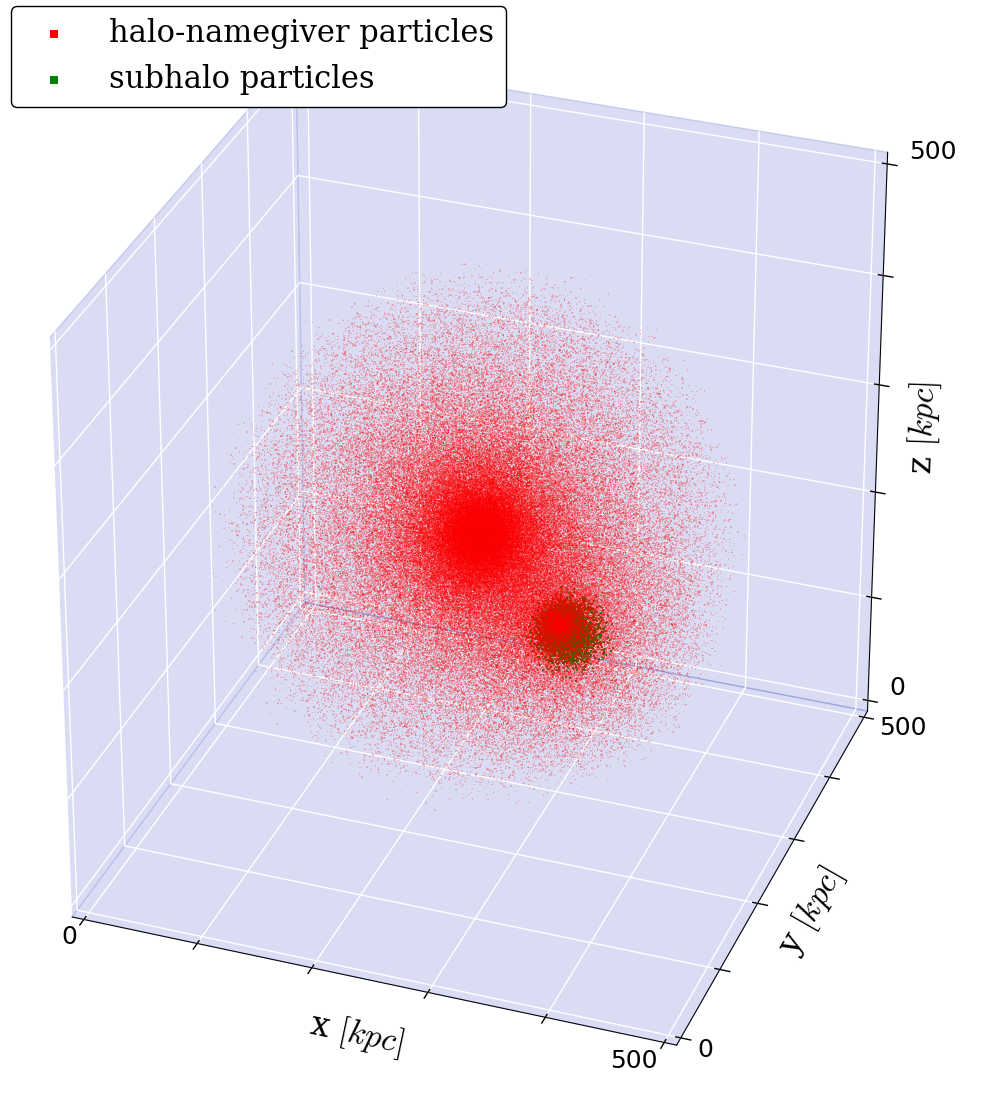
\includegraphics[width = .42\textwidth]{images/dice-two/dice-two-plot-halo1451-saddle.png}} \hspace*{-1em} 	& 
			{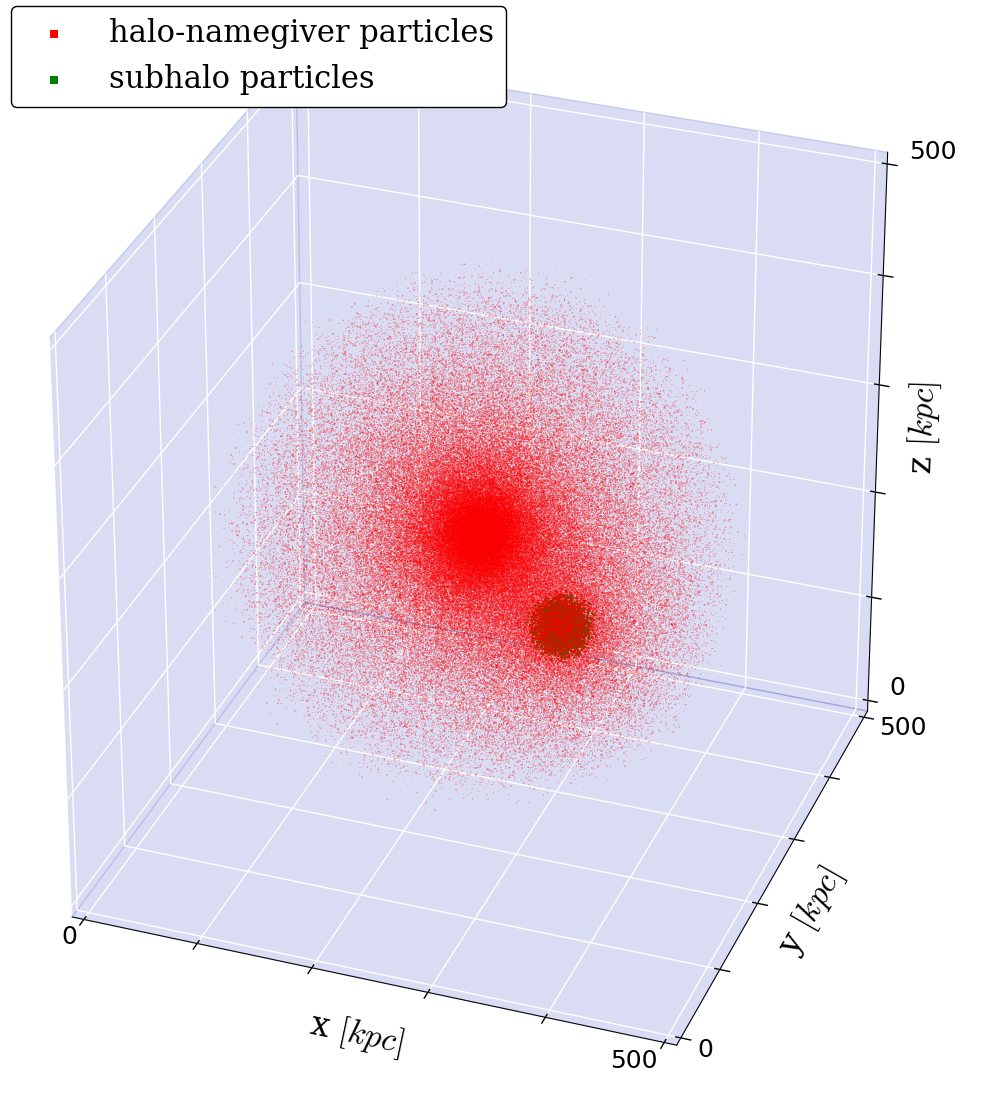
\includegraphics[width = .42\textwidth]{images/dice-two/dice-two-plot-halo1451-iter.png}} \hspace*{-1em}	\\
			%
			%
			\begin{sideways}{ \hspace{.5cm}\textbf{Halo-namegiver particles only} }\end{sideways}	 \hspace*{-1em}			 &			 
			{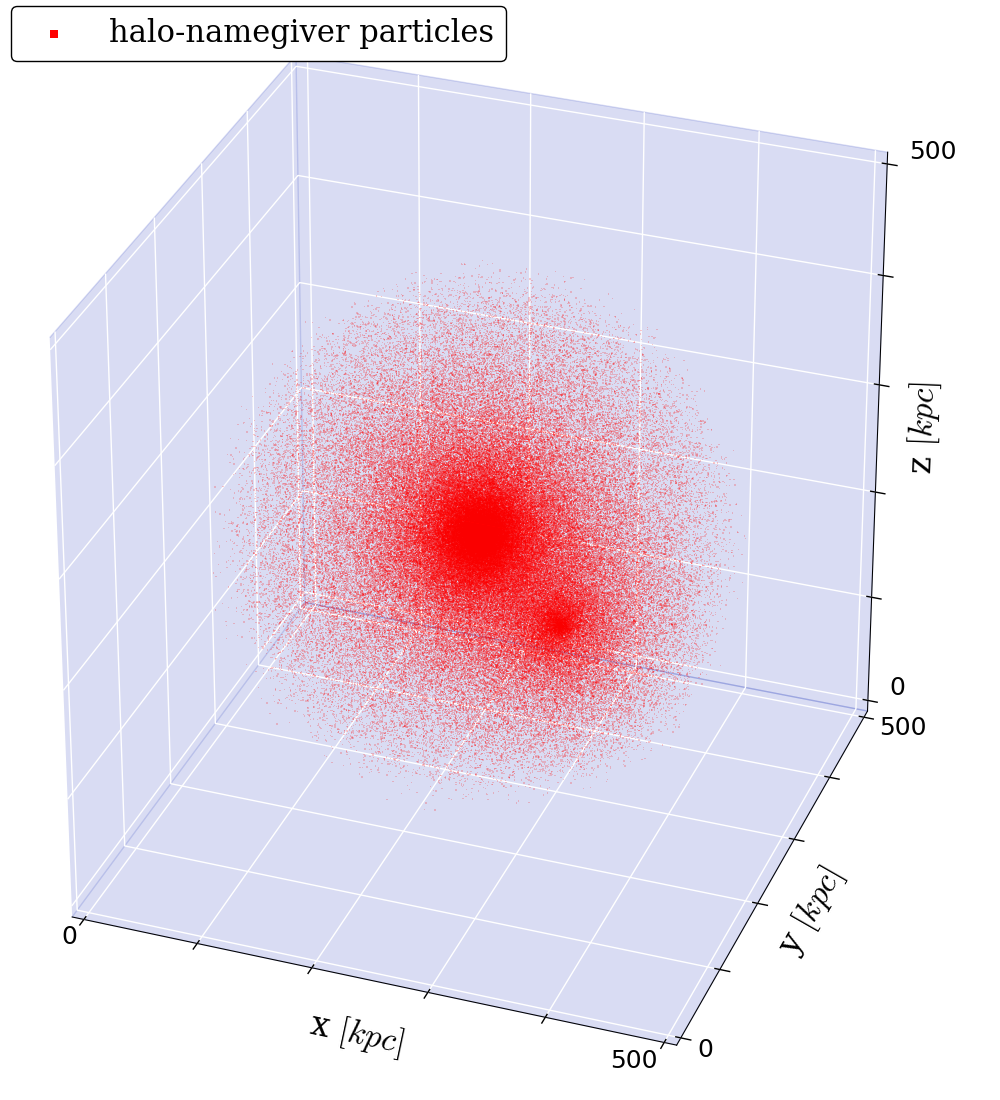
\includegraphics[width = .42\textwidth]{images/dice-two/dice-two-halo-only-saddle.png}} \hspace*{-1em} 		&
			{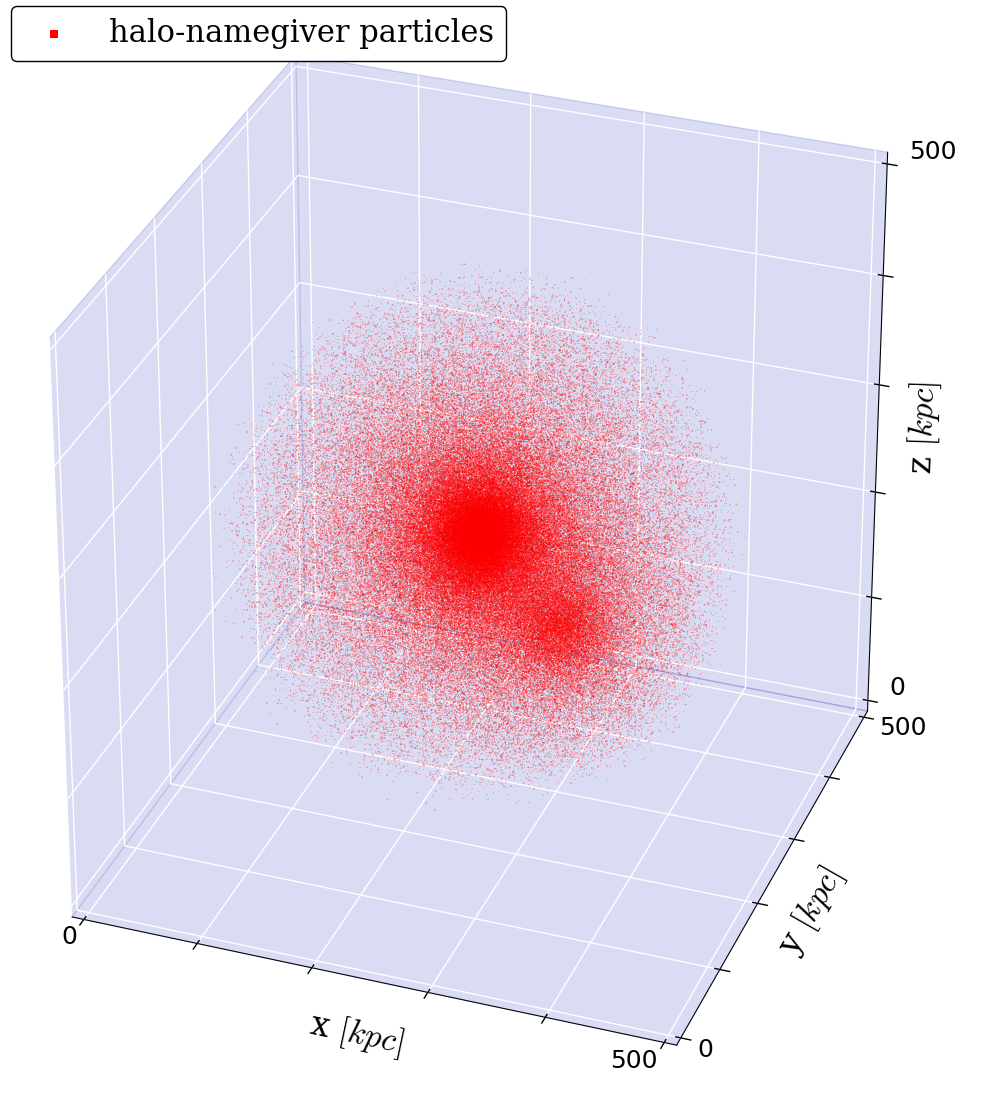
\includegraphics[width = .42\textwidth]{images/dice-two/dice-two-halo-only-iter.png}} \hspace*{-1em}		\\
			%
			%
			\begin{sideways}{ \hspace{2cm}\textbf{Subhalo particles only} }\end{sideways}	 \hspace*{-1em}			 &
			{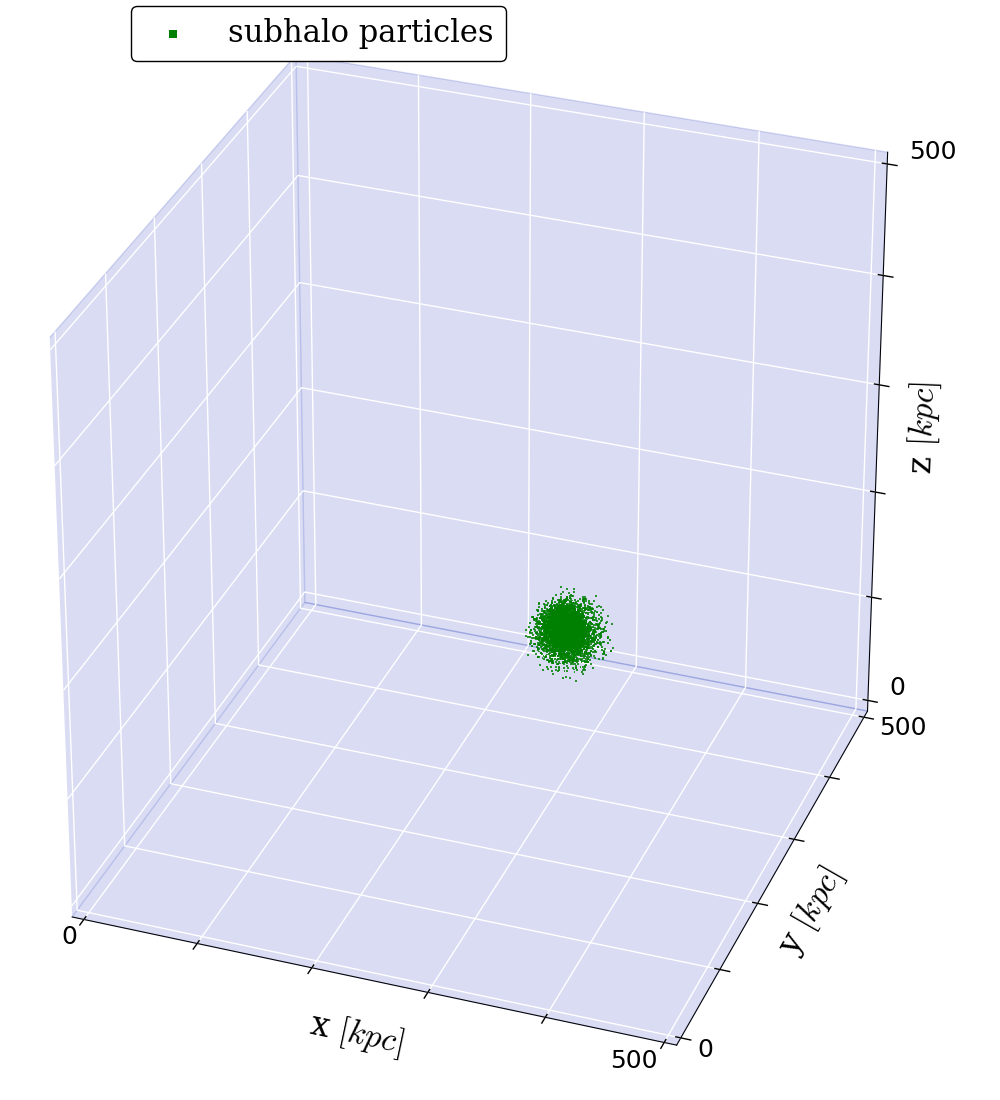
\includegraphics[width = .42\textwidth]{images/dice-two/dice-two-plot-subhalo-saddle.png}} &
			{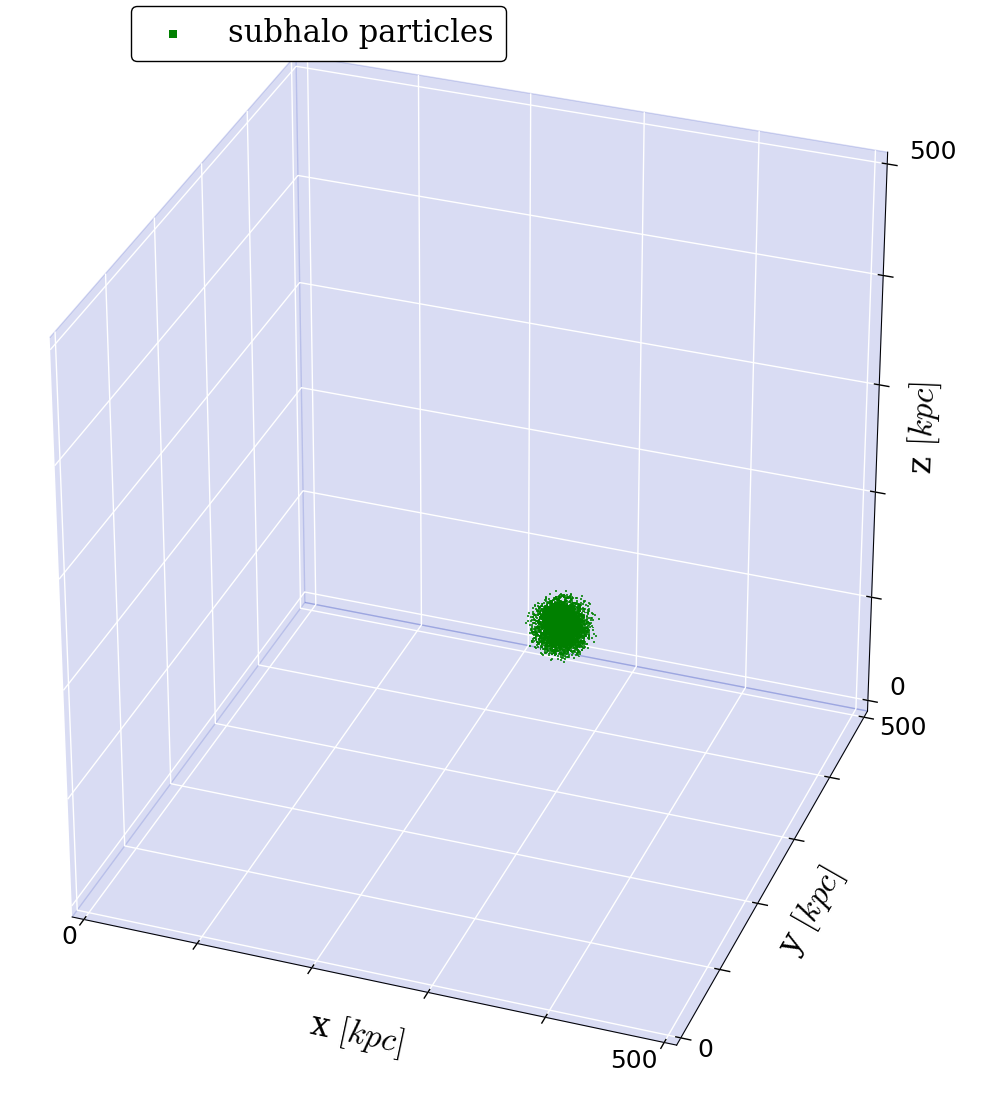
\includegraphics[width = .42\textwidth]{images/dice-two/dice-two-plot-subhalo-iter.png}} \\
			\hline
		\end{tabular}
		\caption{\label{fig:dice_two_results_b}
			The results of \neigh\ and \iter\ unbinding of the \dt-dataset: All particles, halo-namegiver particles only and subhalo particles only.
			}
		}
	\end{figure}
	\label{fig:dice_two_results}
\end{subfigures}







%=====================
% Dice Sub
%=====================

\begin{subfigures}

	\begin{figure}[!htbp]
		{
			\renewcommand{\arraystretch}{0.1}
			\centering	
			%	\subfloat[]{
			\begin{tabular}{|p{.5cm} c c|}
				\hline
				&&\\[1em]
				&	\phewon\ 	& \simple \\[1.5em]
				%
				%
				\begin{sideways}{\hspace{3cm} \textbf{All particles}}\end{sideways} \hspace*{-1em}	&		 
				{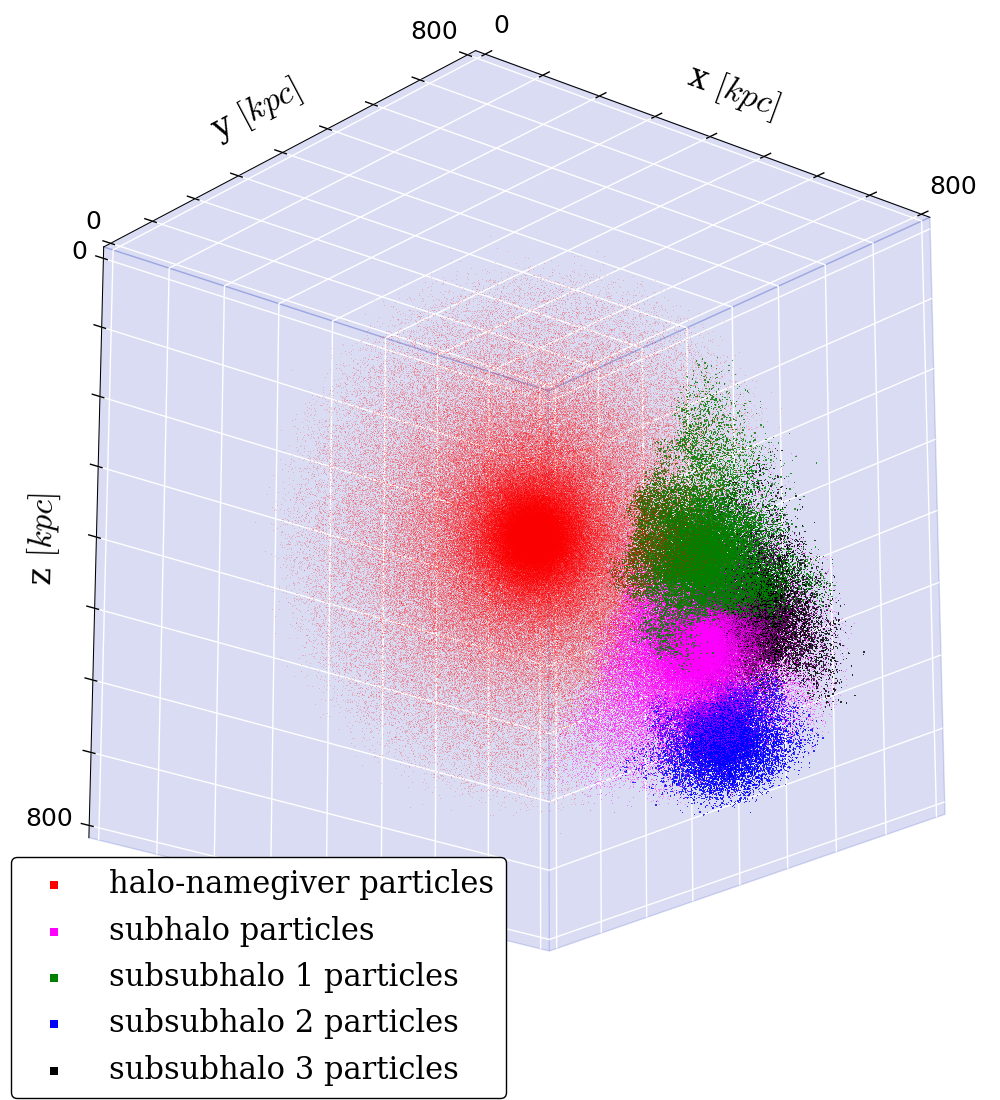
\includegraphics[width = .42\textwidth]{images/dice-sub/dice-sub-plot-halo1-phew.png}} \hspace*{-1em} 	& 
				{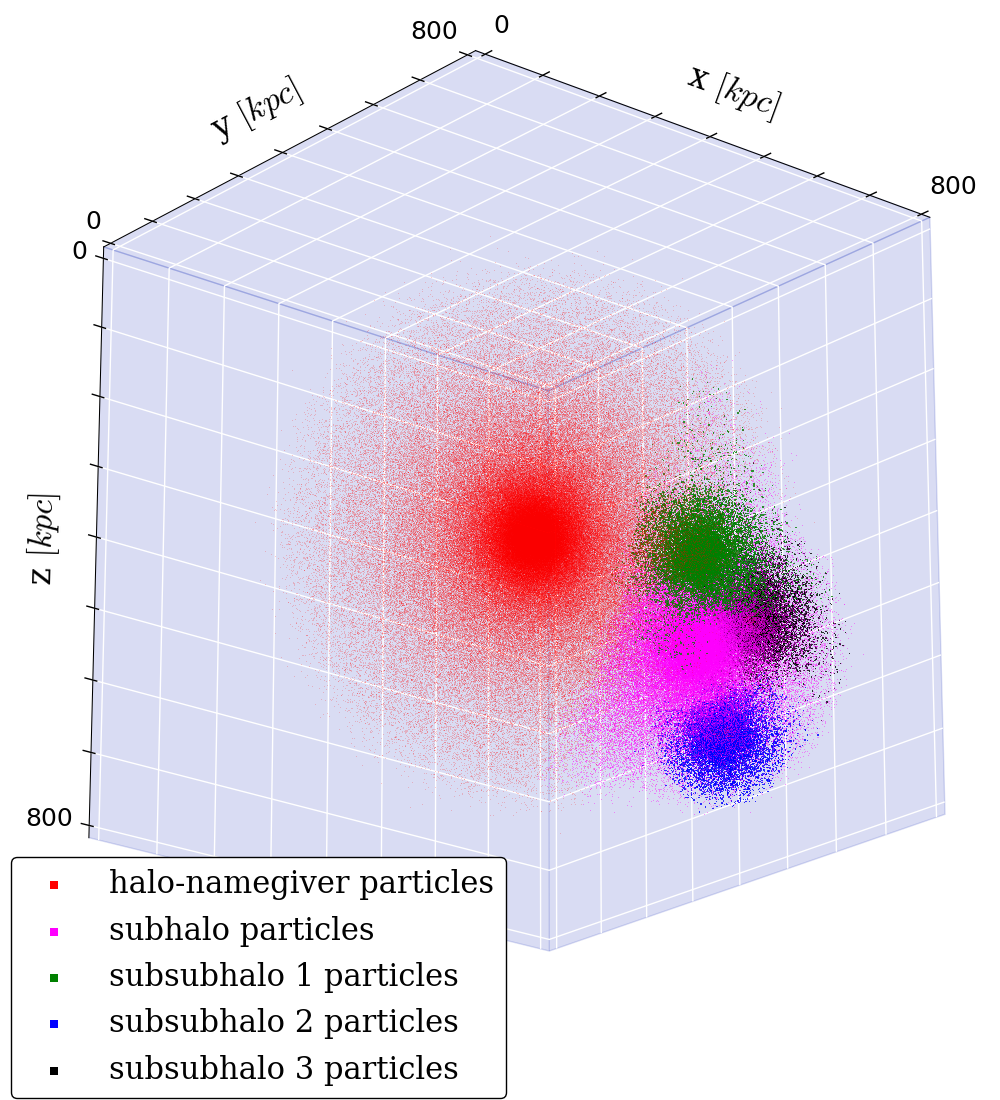
\includegraphics[width = .42\textwidth]{images/dice-sub/dice-sub-plot-halo1-nosaddle.png}} \hspace*{-1em}	\\
				%
				%
				\begin{sideways}{ \hspace{.5cm}\textbf{Halo-namegiver particles only} }\end{sideways}	 \hspace*{-1em}			 &			 
				{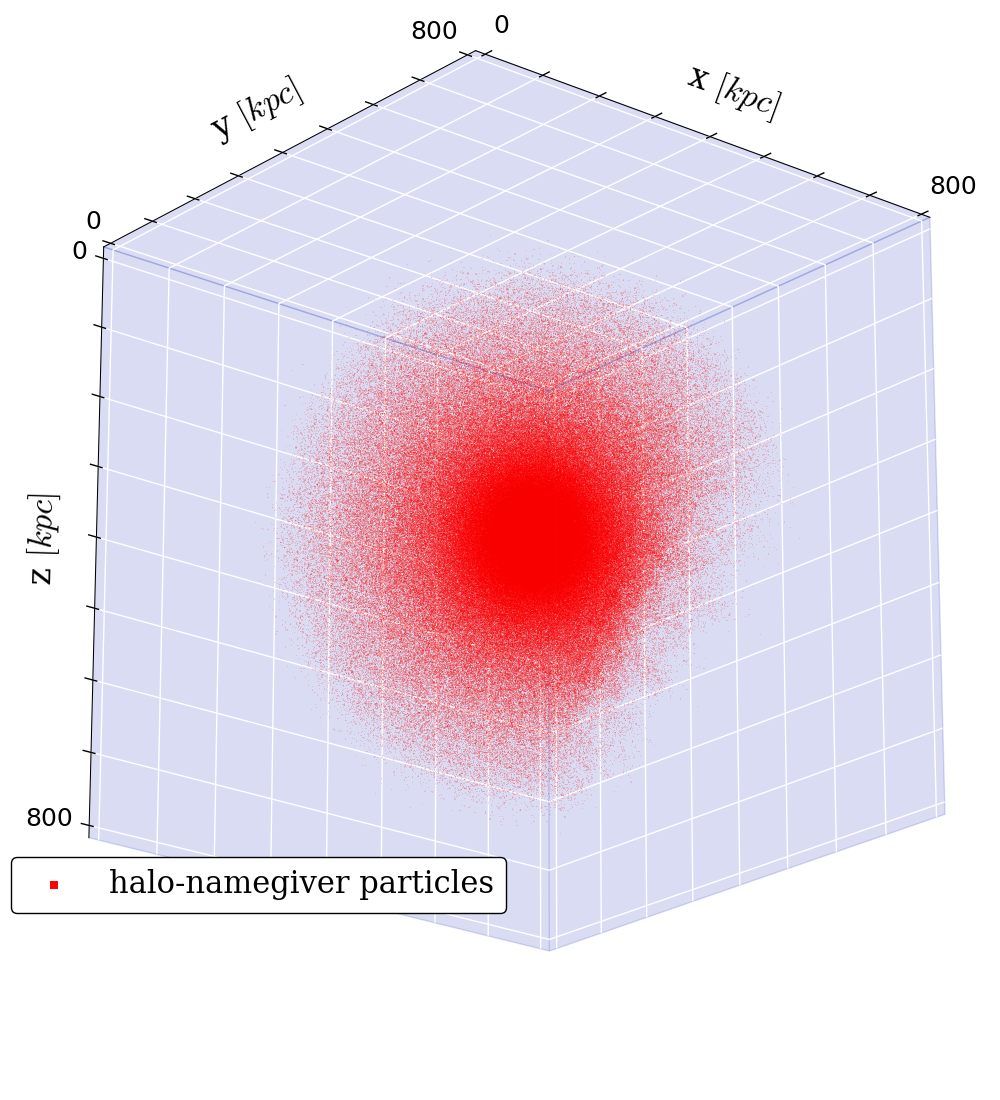
\includegraphics[width = .42\textwidth]{images/dice-sub/dice-sub-halo-only-phew.png}} \hspace*{-1em} 		&
				{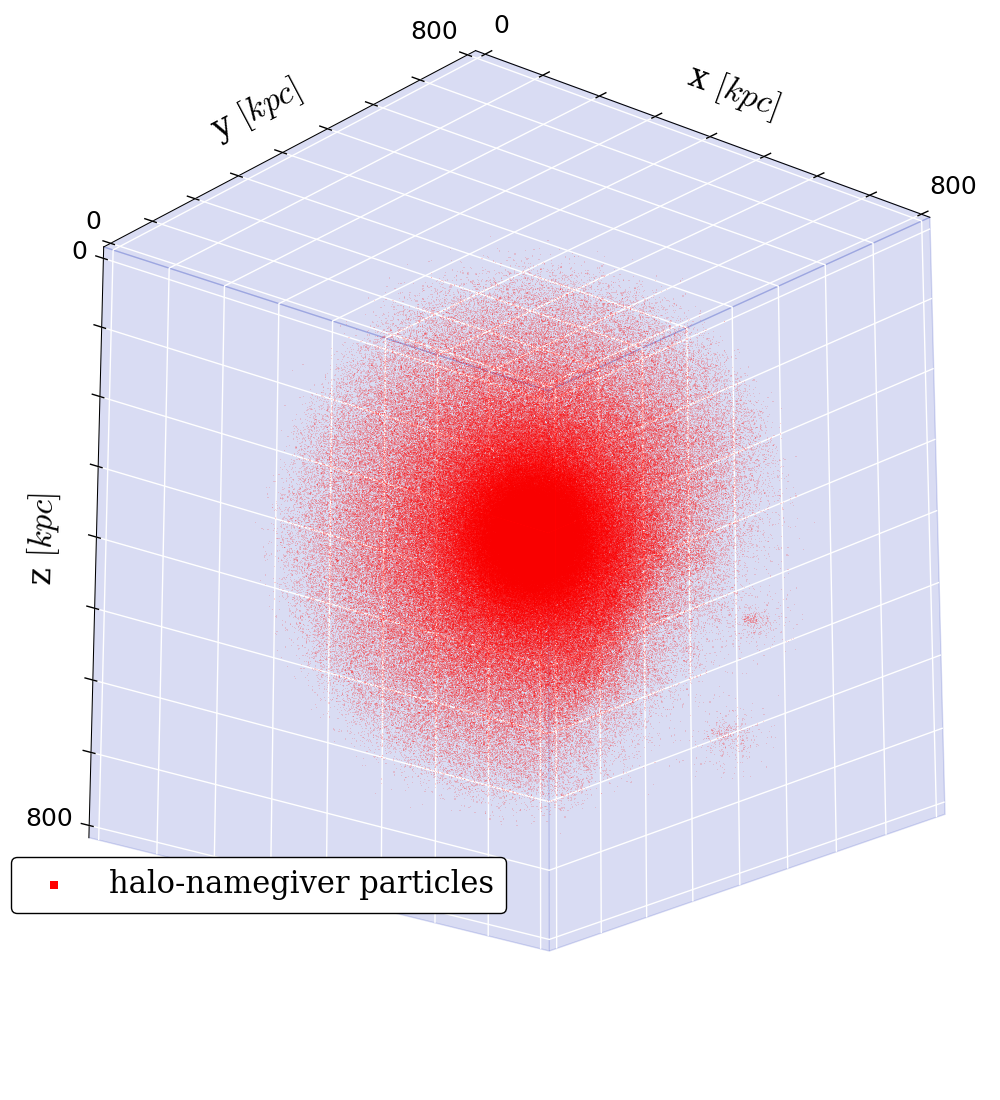
\includegraphics[width = .42\textwidth]{images/dice-sub/dice-sub-halo-only-nosaddle.png}} \hspace*{-1em}		\\
				%
				%
				\begin{sideways}{ \hspace{2cm}\textbf{Subhalo particles only} }\end{sideways}	 \hspace*{-1em}			 &
				{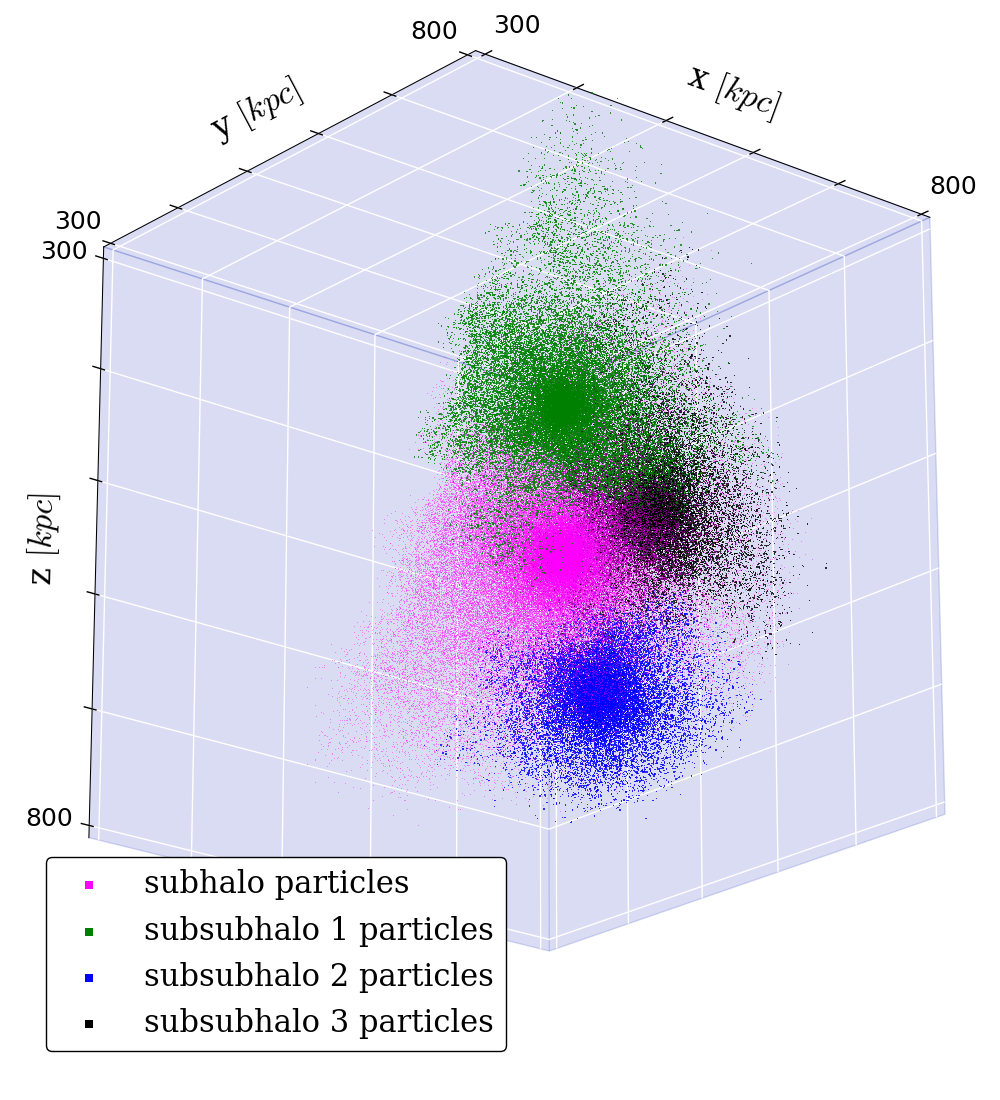
\includegraphics[width = .42\textwidth]{images/dice-sub/dice-sub-plot-subclumps-phew.png}} &
				{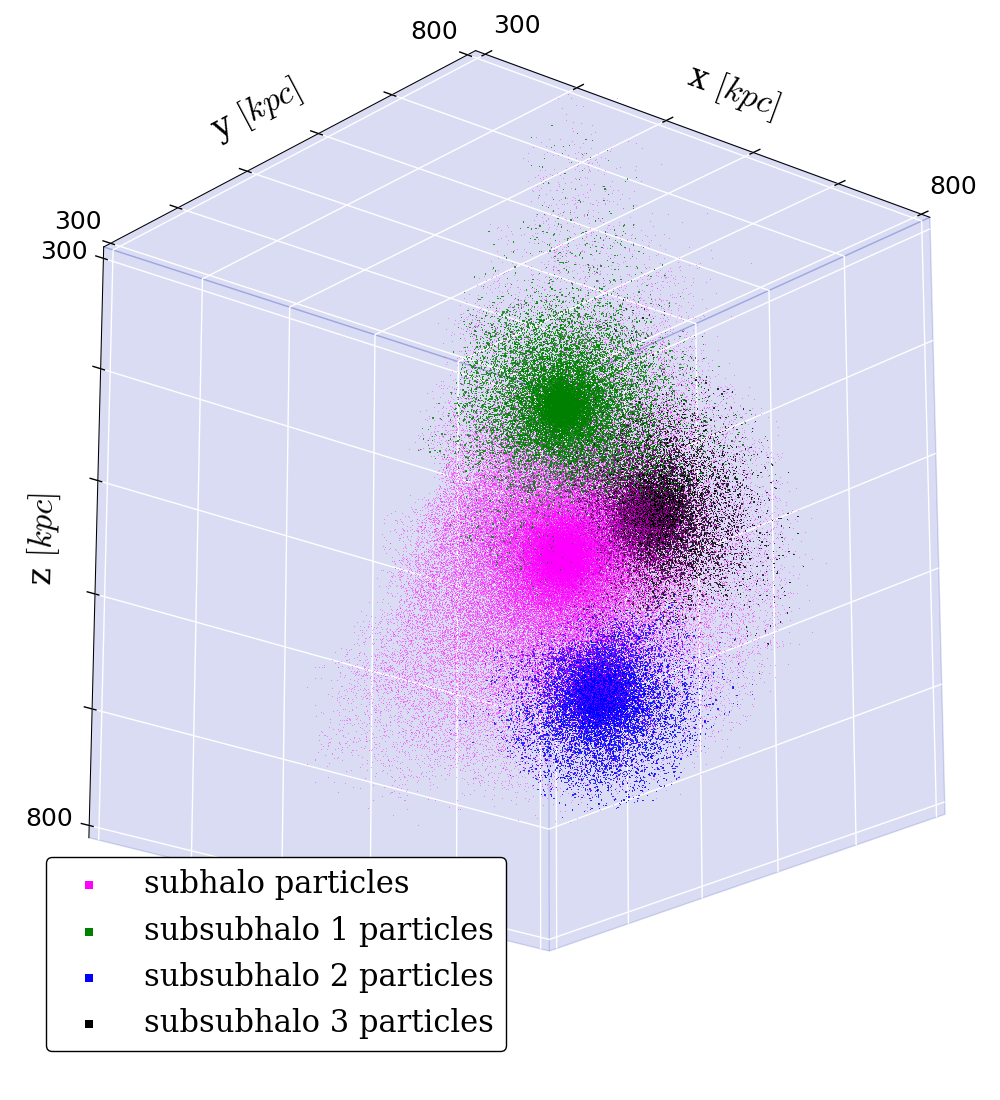
\includegraphics[width = .42\textwidth]{images/dice-sub/dice-sub-plot-subclumps-nosaddle.png}} \\
				\hline
			\end{tabular}
			\caption{\label{fig:dice_sub_results_a}The results of \phewon\ and \simple\ unbinding of the \ds-dataset: All particles, halo-namegiver particles only and subhalo particles only.}
		}
	\end{figure}
	%=================================================
	%=================================================
	%=================================================
	\begin{figure}[!htbp]%\ContinuedFloat
		{
			\renewcommand{\arraystretch}{0.1}
			\centering	
			\begin{tabular}{|p{.5cm} c c|}
				\hline
				&&\\[1em]
				&	\neigh\ 	& \iter \\[1.5em]
				%
				%
				\begin{sideways}{\hspace{3cm} \textbf{All particles}}\end{sideways} \hspace*{-1em}	&		 
				{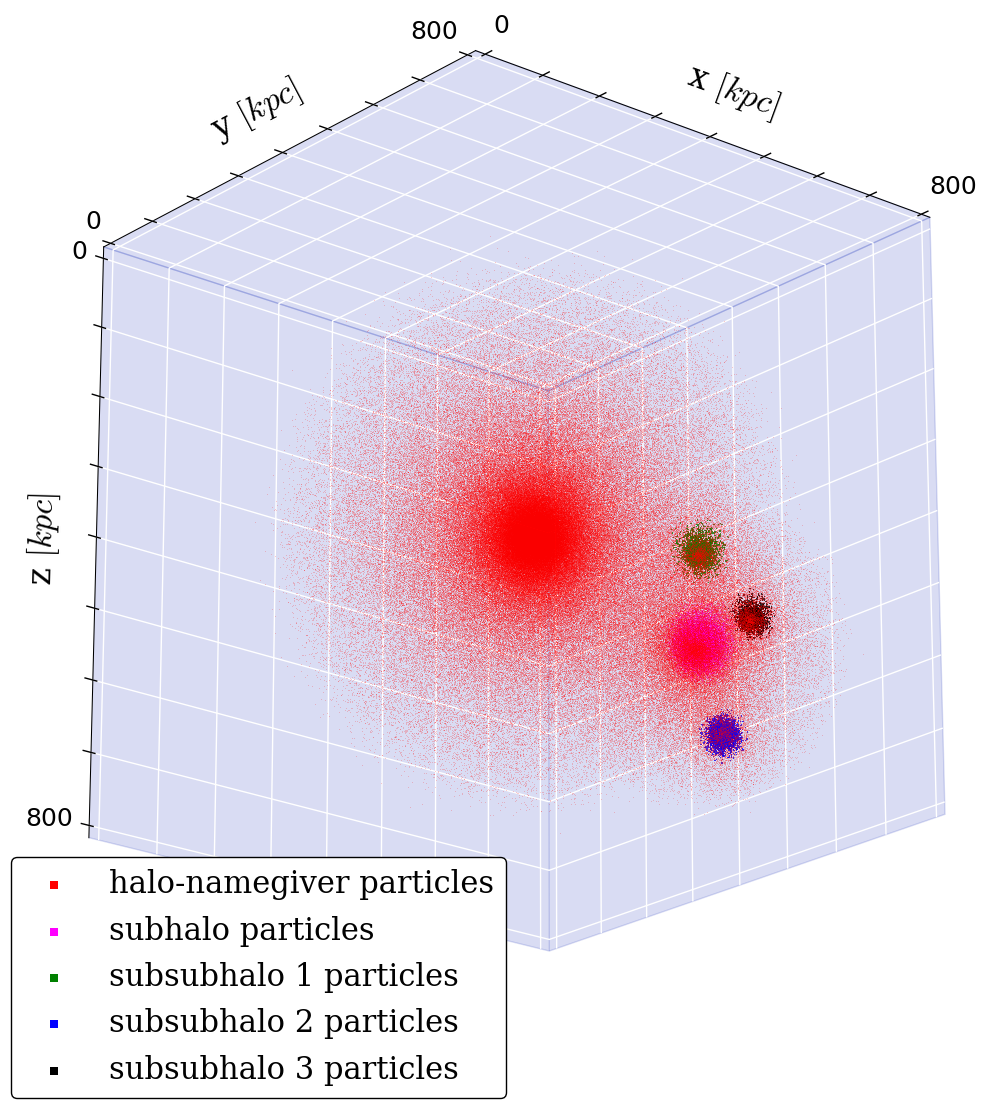
\includegraphics[width = .42\textwidth]{images/dice-sub/dice-sub-plot-halo1-saddle.png}} \hspace*{-1em} 	& 
				{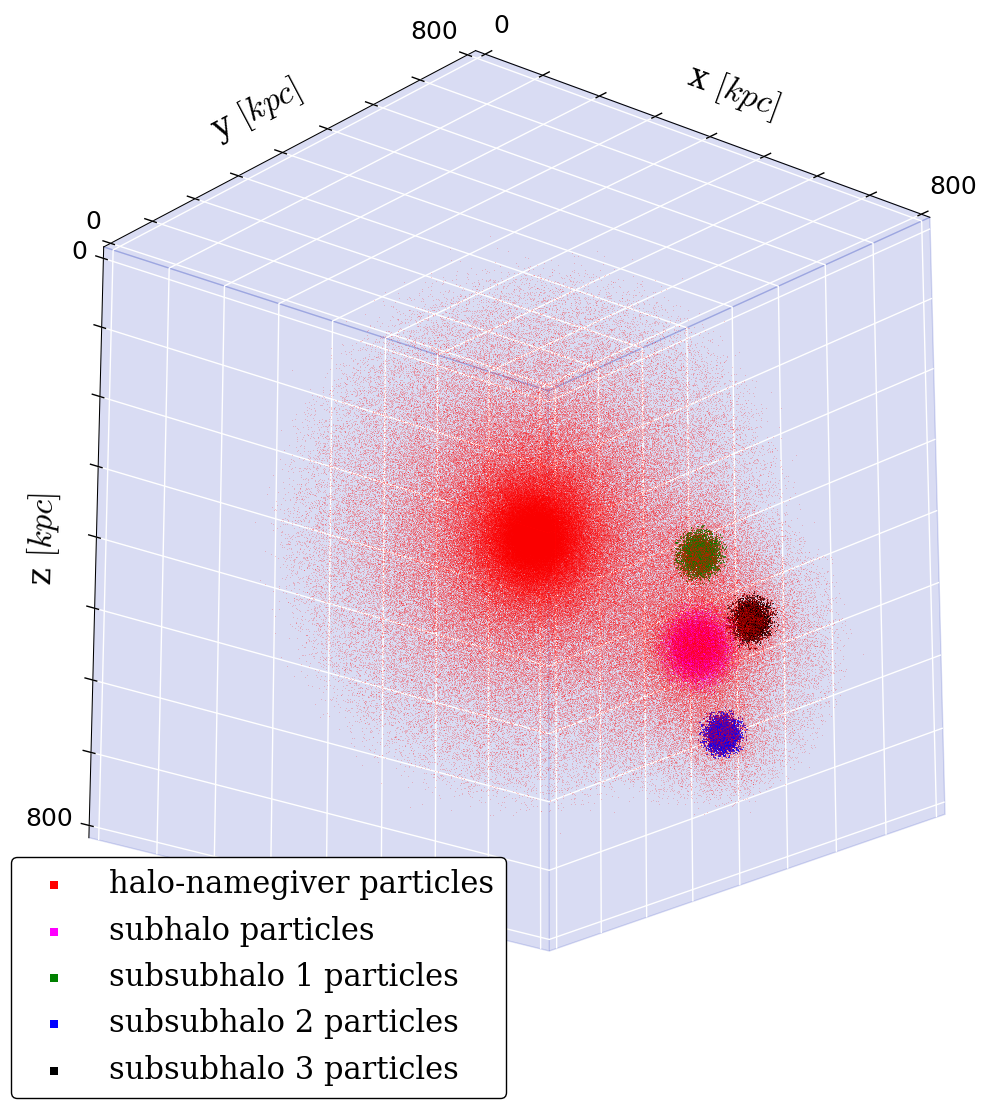
\includegraphics[width = .42\textwidth]{images/dice-sub/dice-sub-plot-halo1-iter.png}} \hspace*{-1em}	\\
				%
				%
				\begin{sideways}{ \hspace{.5cm}\textbf{Halo-namegiver particles only} }\end{sideways}	 \hspace*{-1em}			 &			 
				{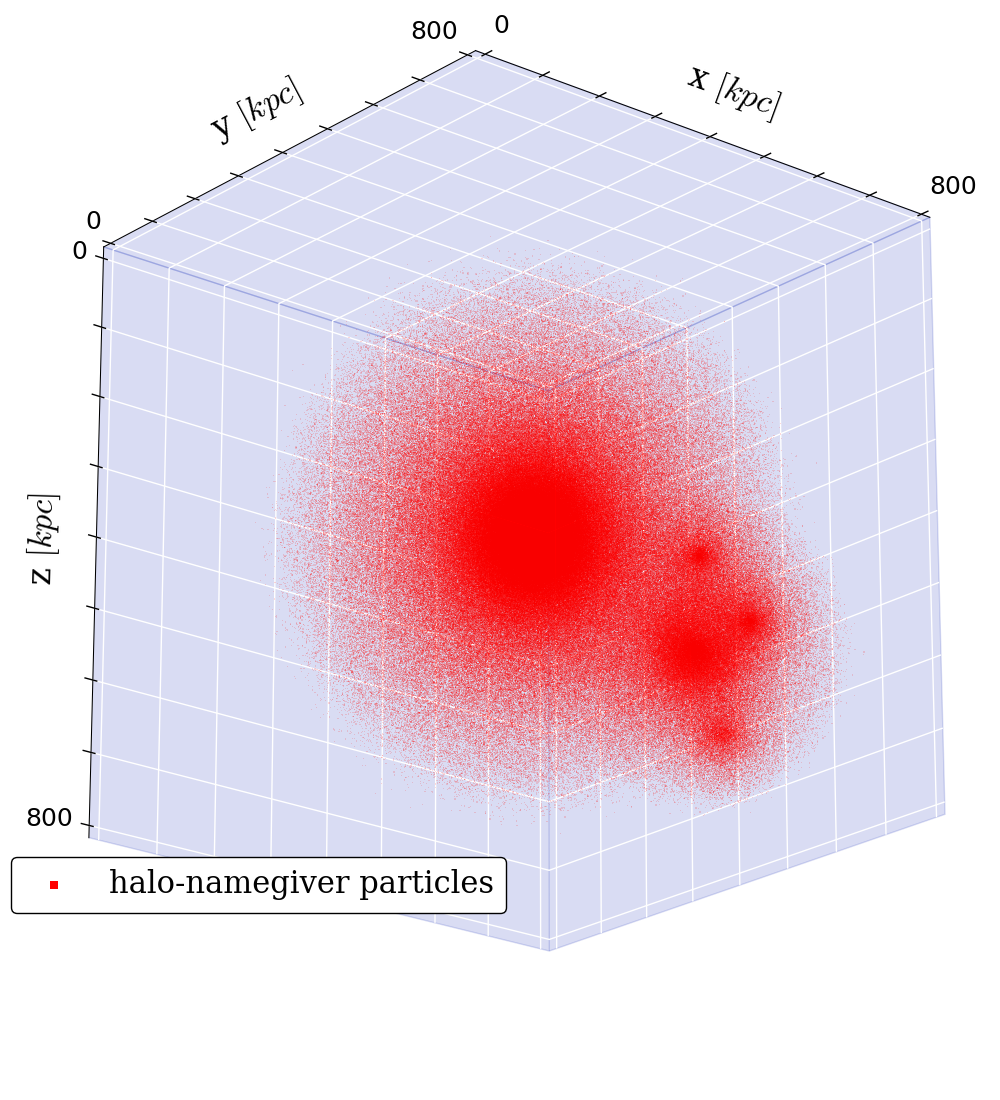
\includegraphics[width = .42\textwidth]{images/dice-sub/dice-sub-halo-only-saddle.png}} \hspace*{-1em} 		&
				{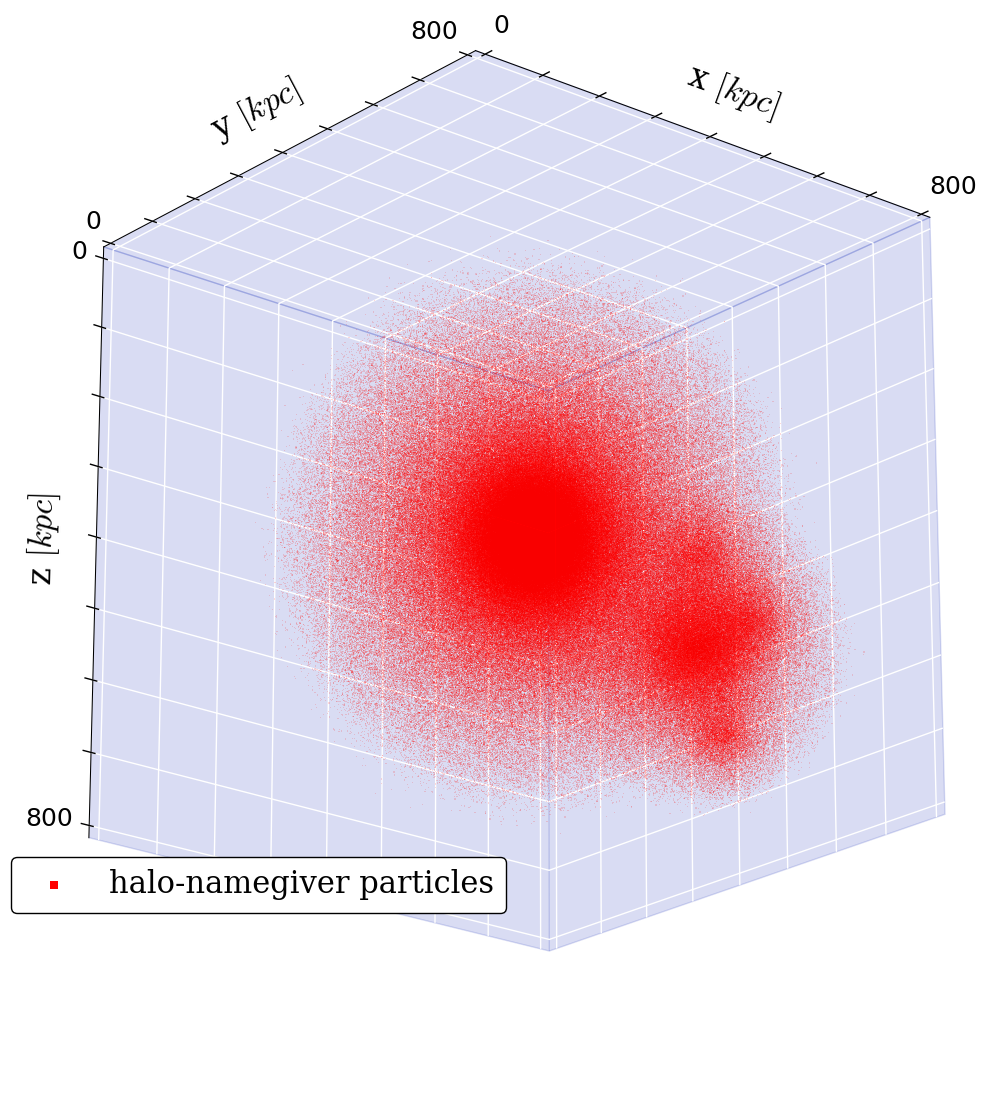
\includegraphics[width = .42\textwidth]{images/dice-sub/dice-sub-halo-only-iter.png}} \hspace*{-1em}		\\
				%
				%
				\begin{sideways}{ \hspace{2cm}\textbf{Subhalo particles only} }\end{sideways}	 \hspace*{-1em}			 &
				{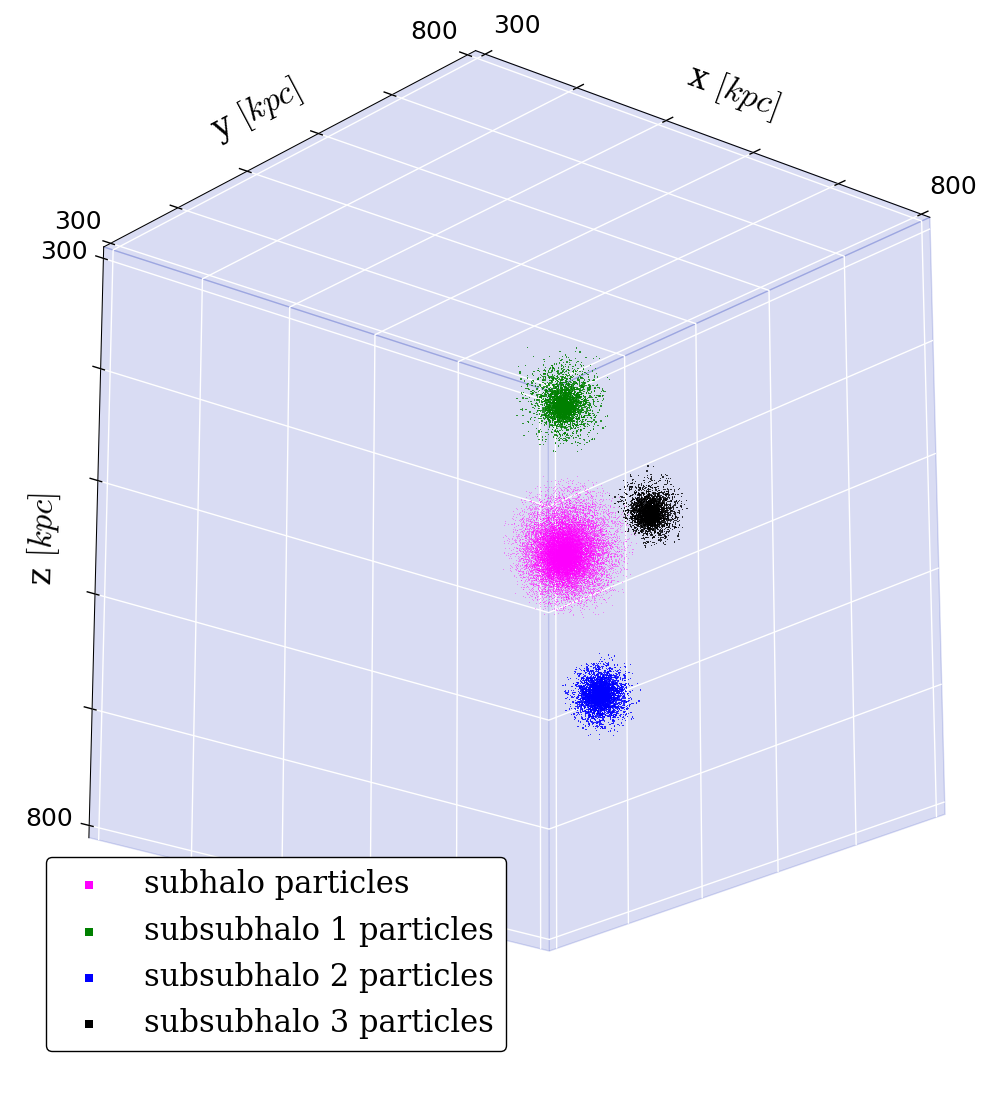
\includegraphics[width = .42\textwidth]{images/dice-sub/dice-sub-plot-subclumps-saddle.png}} &
				{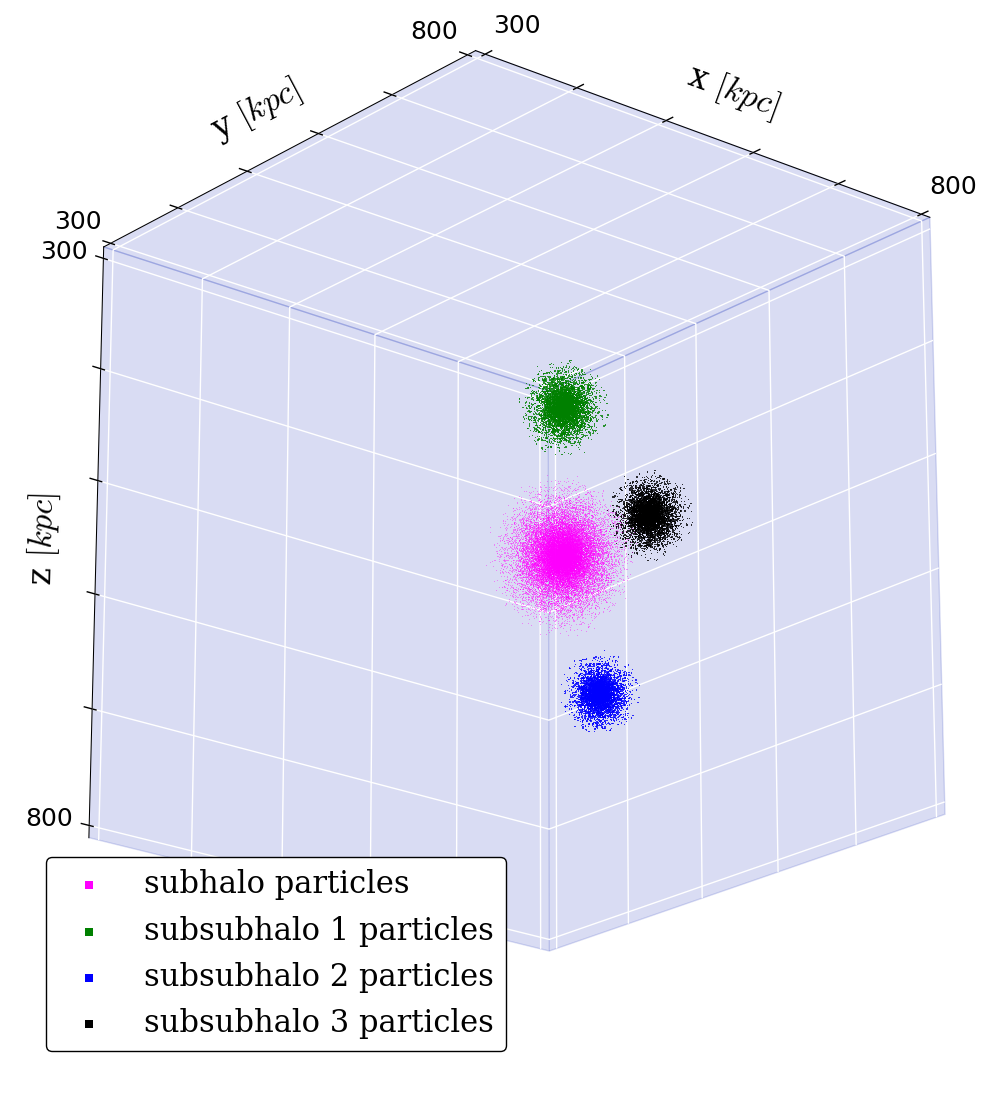
\includegraphics[width = .42\textwidth]{images/dice-sub/dice-sub-plot-subclumps-iter.png}} \\
				\hline
			\end{tabular}
			\caption{\label{fig:dice_sub_results_b}
				The results of \neigh\ and \iter\ unbinding of the \ds-dataset: All particles, halo-namegiver particles only and subhalo particles only.
			}
		}
	\end{figure}
	\label{fig:dice_sub_results}
\end{subfigures}




























































%\begin{sidewaysfigure}[!htbp]
%	{\renewcommand{\arraystretch}{0.1}
%		
%	\subfloat[The results of \phewon\ and \simple\ unbinding of the \ds-dataset: All particles, halo-namegiver particles only and subclumps particles only.]{
%		\begin{tabular}{|p{1cm} c c c|}
%			\hline
%			&&&\\[1em]
%													&
%			\textbf{All particles} 					&
%			\textbf{Halo-namegiver particles only} 	&
%			\textbf{Subhalo particles only} 		\\[1em]
%			%
%			%
%			\begin{sideways}{\hspace{3cm} \phewon}\end{sideways} \hspace*{-1em}%		 
%			& {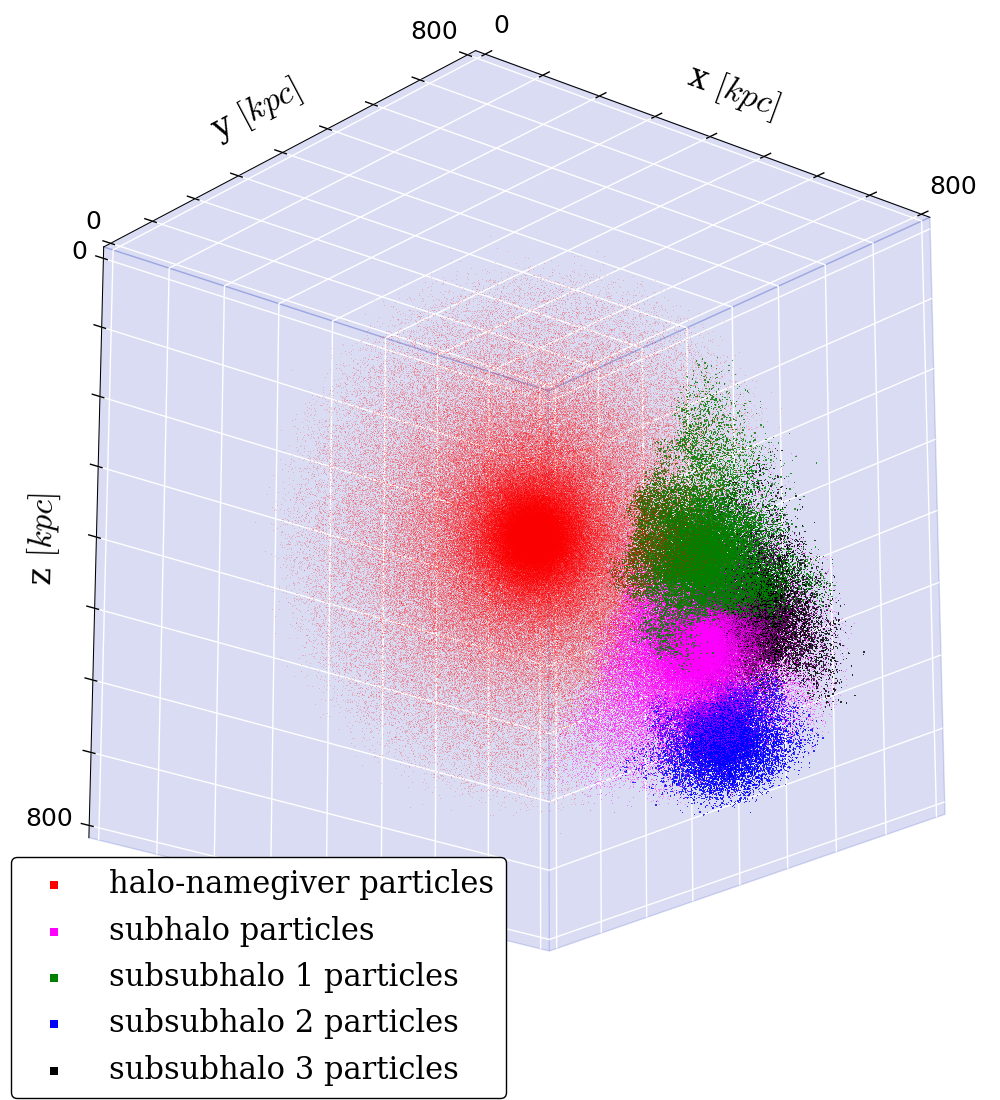
\includegraphics[width = .28\textwidth]{images/dice-sub/dice-sub-plot-halo1-phew.png}} \hspace*{-1em}%
%			 & {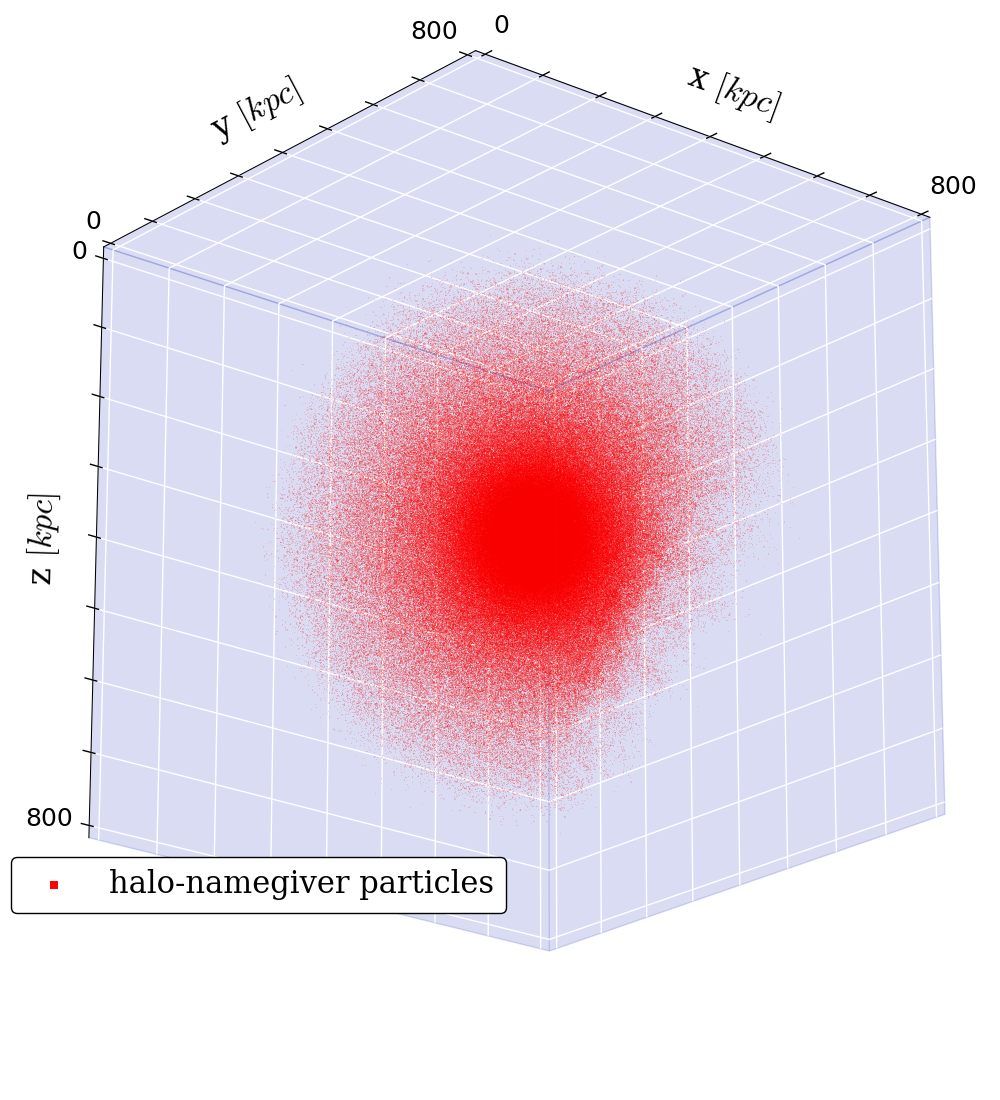
\includegraphics[width = .28\textwidth]{images/dice-sub/dice-sub-halo-only-phew.png}} \hspace*{-1em}% 
%			 &{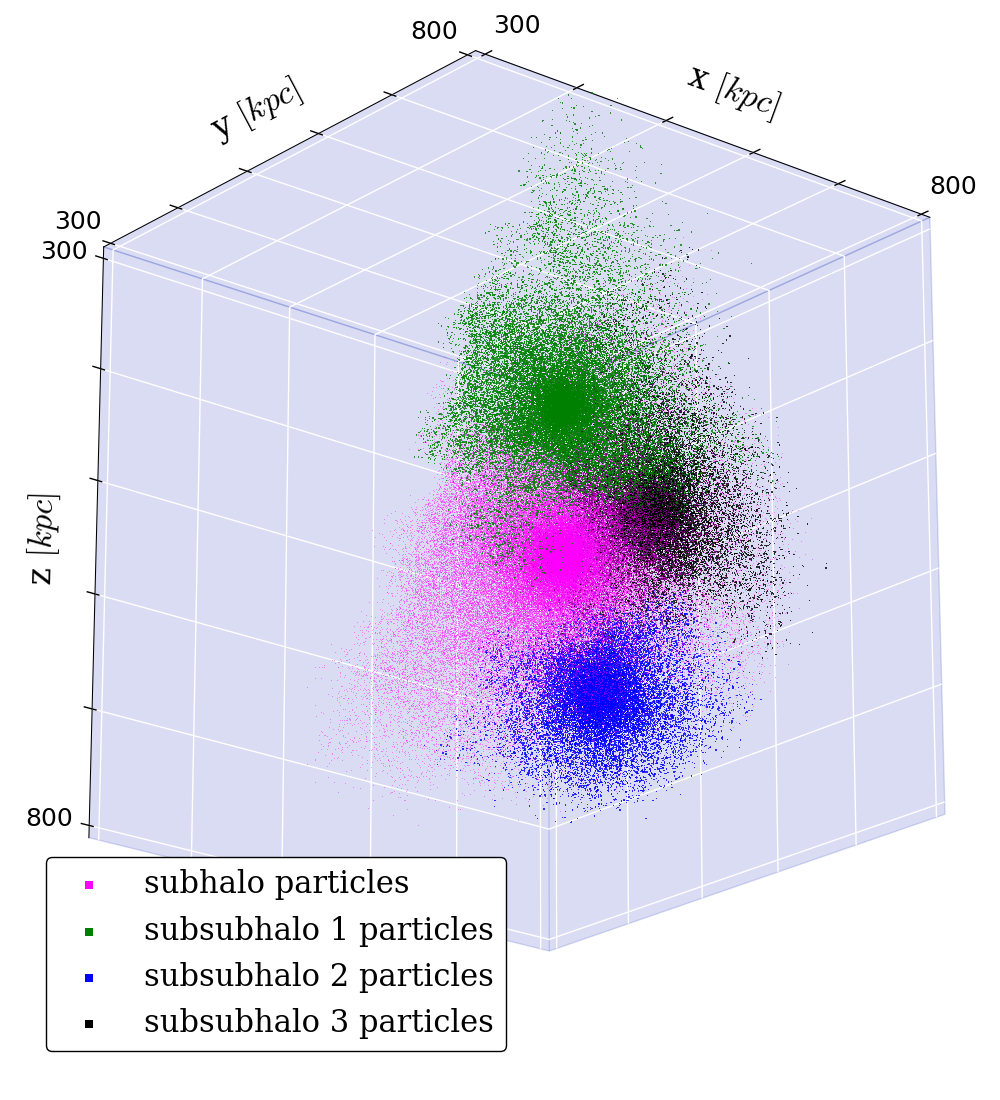
\includegraphics[width = .28\textwidth]{images/dice-sub/dice-sub-plot-subclumps-phew.png}} \\
%			%
%			%
%			\begin{sideways}{ \hspace{3cm}\simple\ unbinding }\end{sideways}	 \hspace*{-1em}			 &
%			{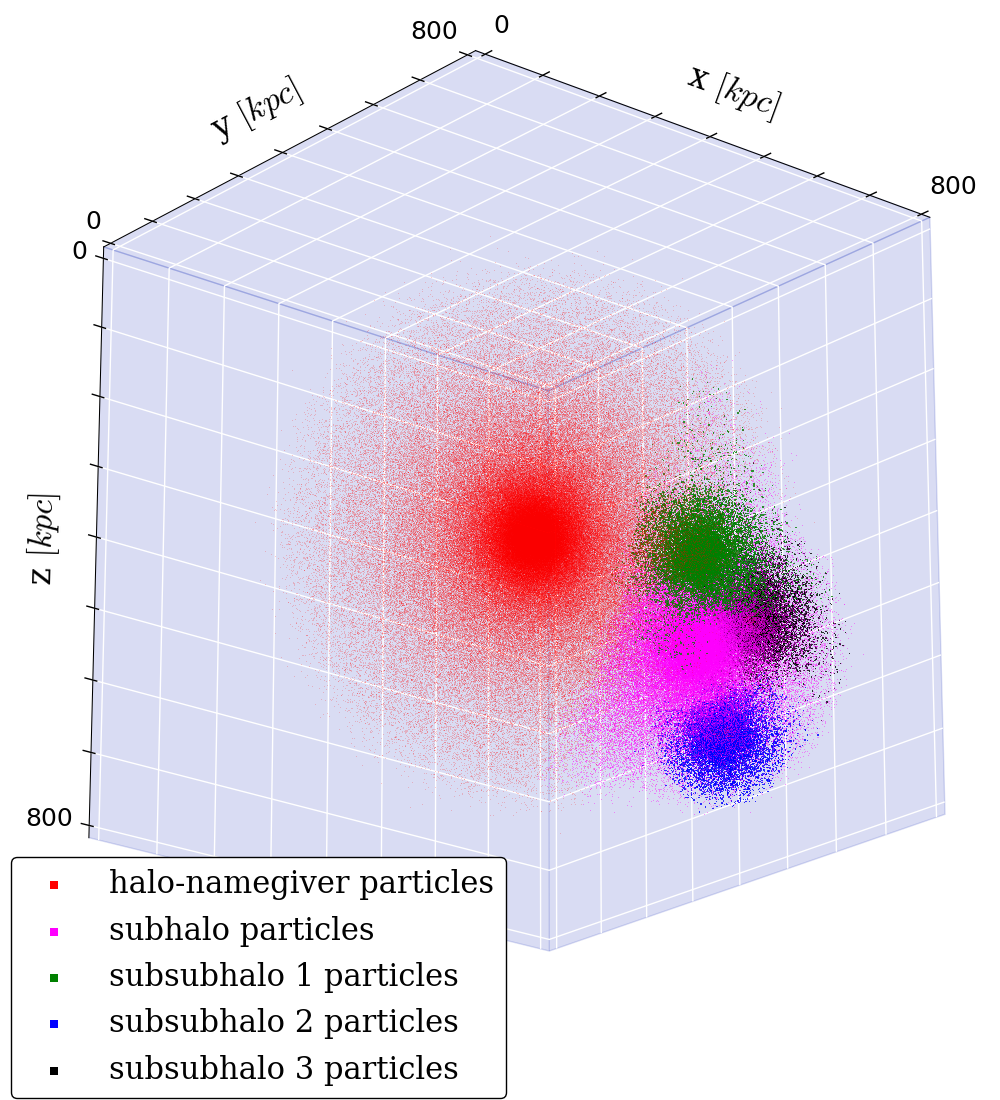
\includegraphics[width = .28\textwidth]{images/dice-sub/dice-sub-plot-halo1-nosaddle.png}} \hspace*{-1em}&
%			{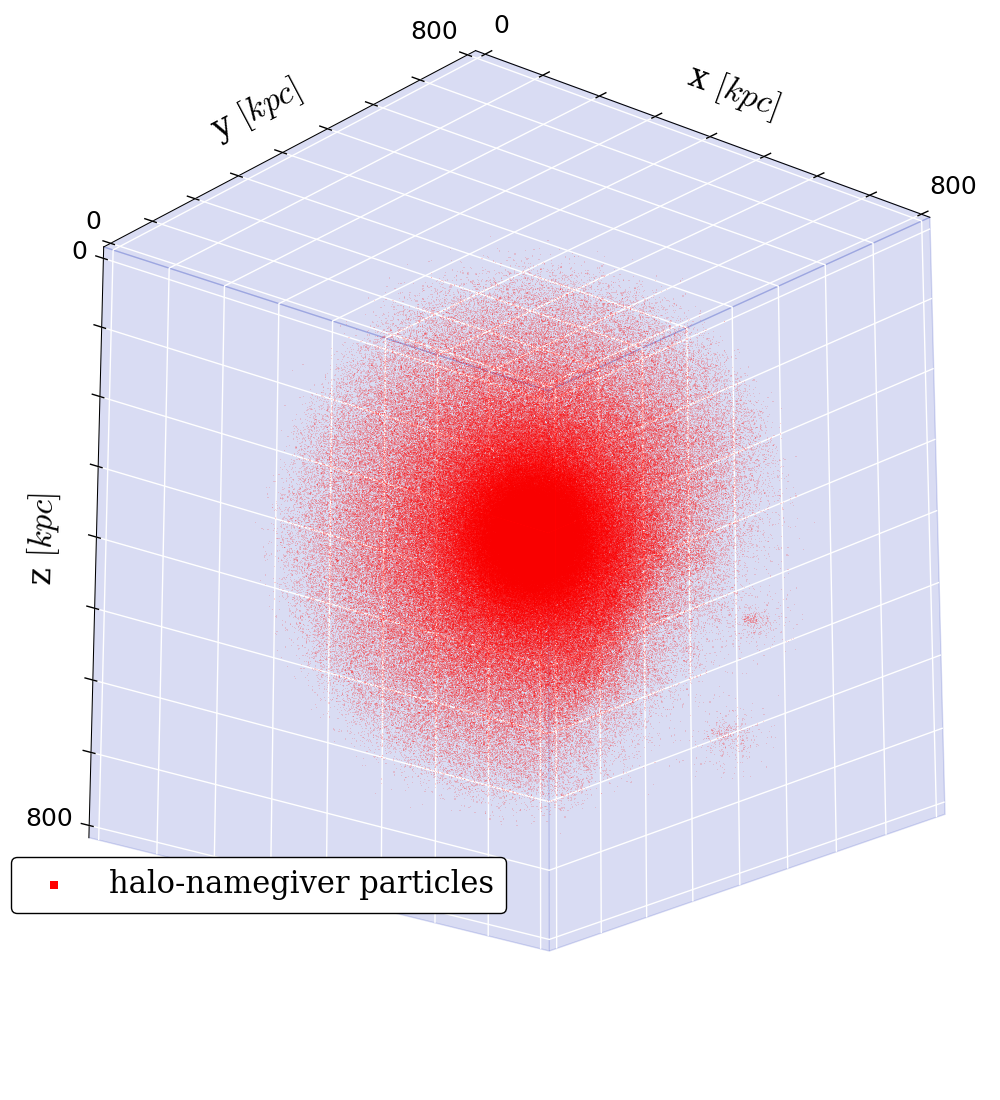
\includegraphics[width = .28\textwidth]{images/dice-sub/dice-sub-halo-only-nosaddle.png}} \hspace*{-1em}&
%			{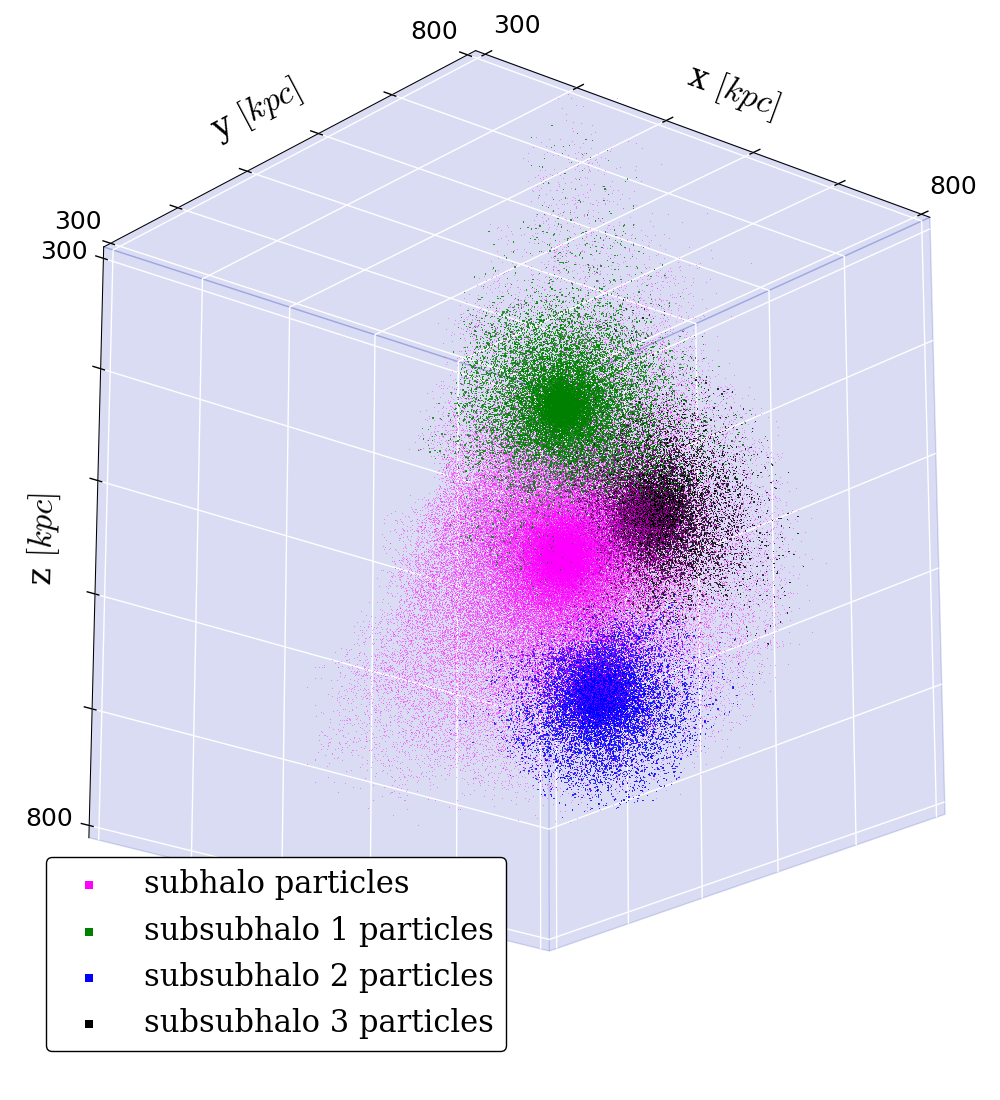
\includegraphics[width = .28\textwidth]{images/dice-sub/dice-sub-plot-subclumps-nosaddle.png}} \\
%			\hline
%		\end{tabular}
%		\label{fig:dice_sub_results_a}
%		}
%	}
%	\phantomcaption
%\end{sidewaysfigure}
%%=================================================
%%=================================================
%%=================================================
%\begin{sidewaysfigure}[!htbp]\ContinuedFloat
%	\footnotesize
%	{\renewcommand{\arraystretch}{0.1}
%	\subfloat[The results of \neigh\ and \iter\ unbinding of the \ds-dataset: All particles, halo-namegiver particles only and subclumps particles only.]{
%		\begin{tabular}{|p{1cm} c c c|}
%			\hline
%			&&&\\[1em]
%													&
%			\textbf{All particles} 					&
%			\textbf{Halo-namegiver particles only} 	&
%			\textbf{Subhalo particles only}			\\[1em]
%			%
%			%
%			\begin{sideways}{ \hspace{3cm}\neigh\ unbinding }\end{sideways}		\hspace*{-1em}		 &		
%			{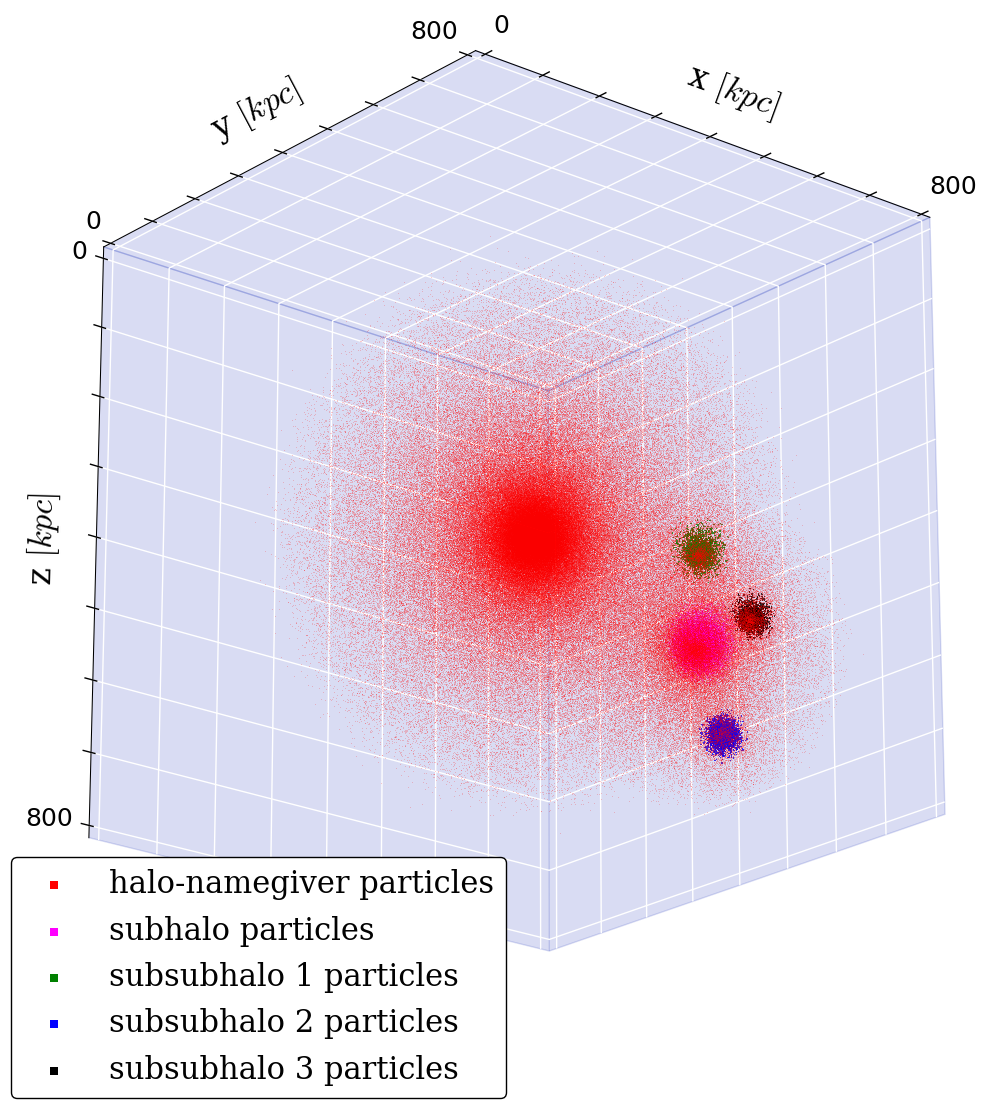
\includegraphics[width = .28\textwidth]{images/dice-sub/dice-sub-plot-halo1-saddle.png}}\hspace*{-1em} &
%			{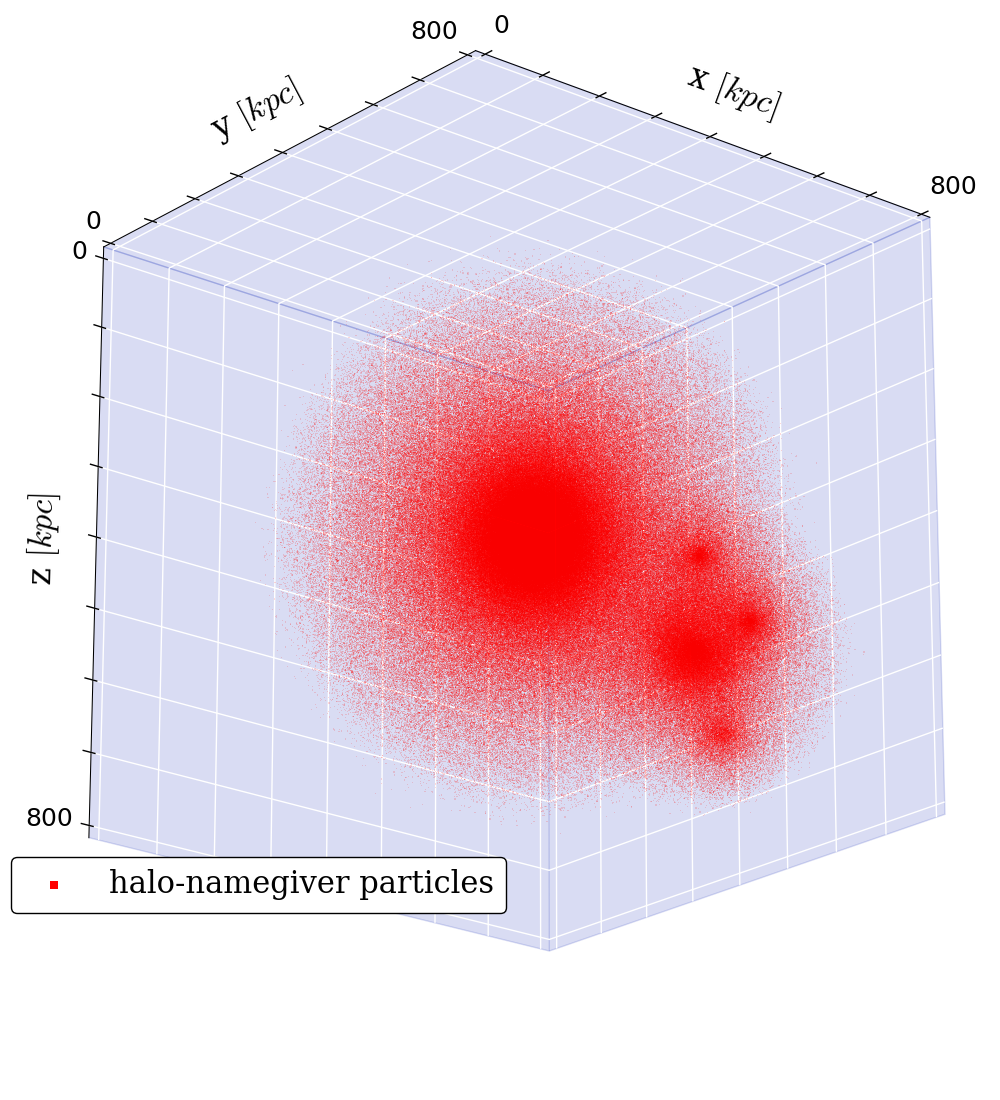
\includegraphics[width = .28\textwidth]{images/dice-sub/dice-sub-halo-only-saddle.png}}\hspace*{-1em} &
%			{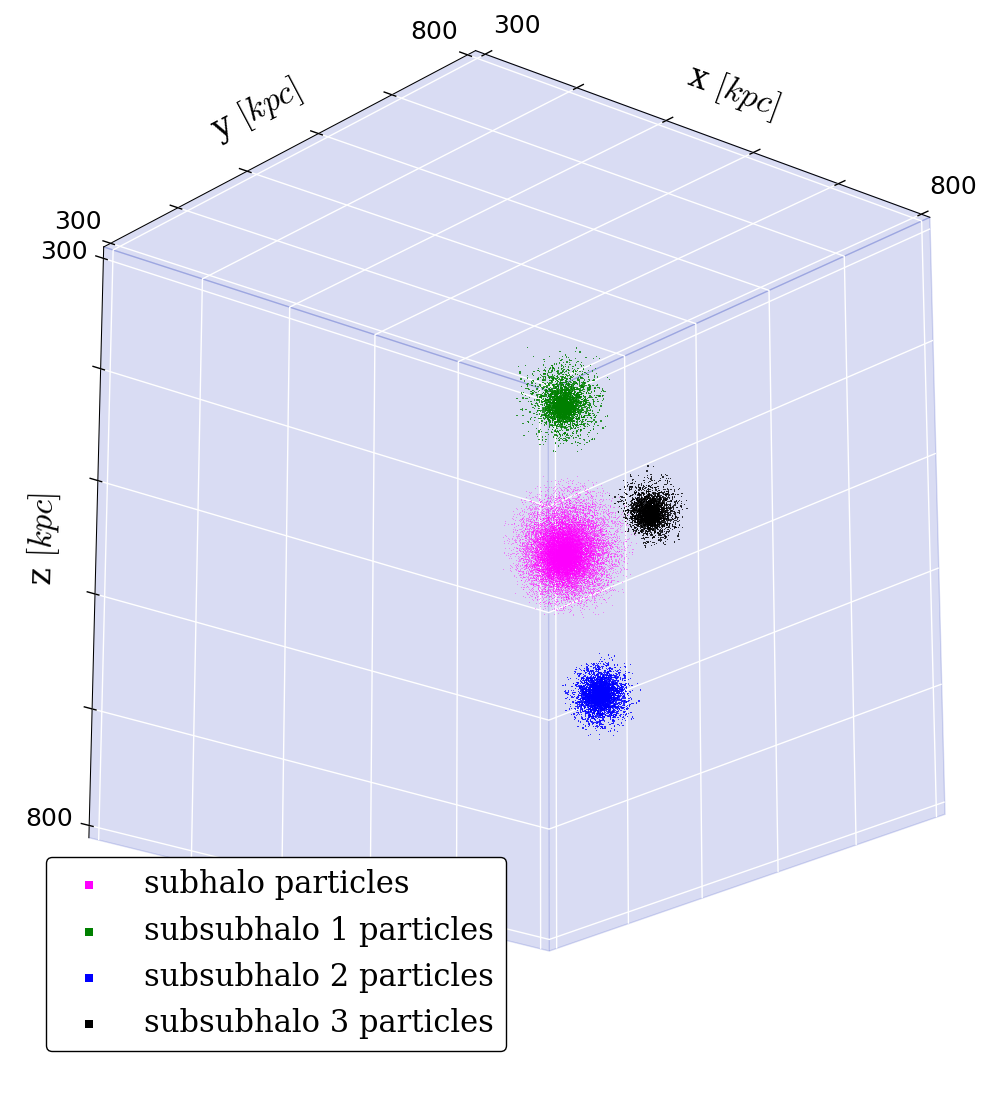
\includegraphics[width = .28\textwidth]{images/dice-sub/dice-sub-plot-subclumps-saddle.png}} \\
%	%		%
%	%		%
%			\begin{sideways}{\hspace{3cm} \iter\ unbinding }\end{sideways}		\hspace*{-1em}		 &		
%			{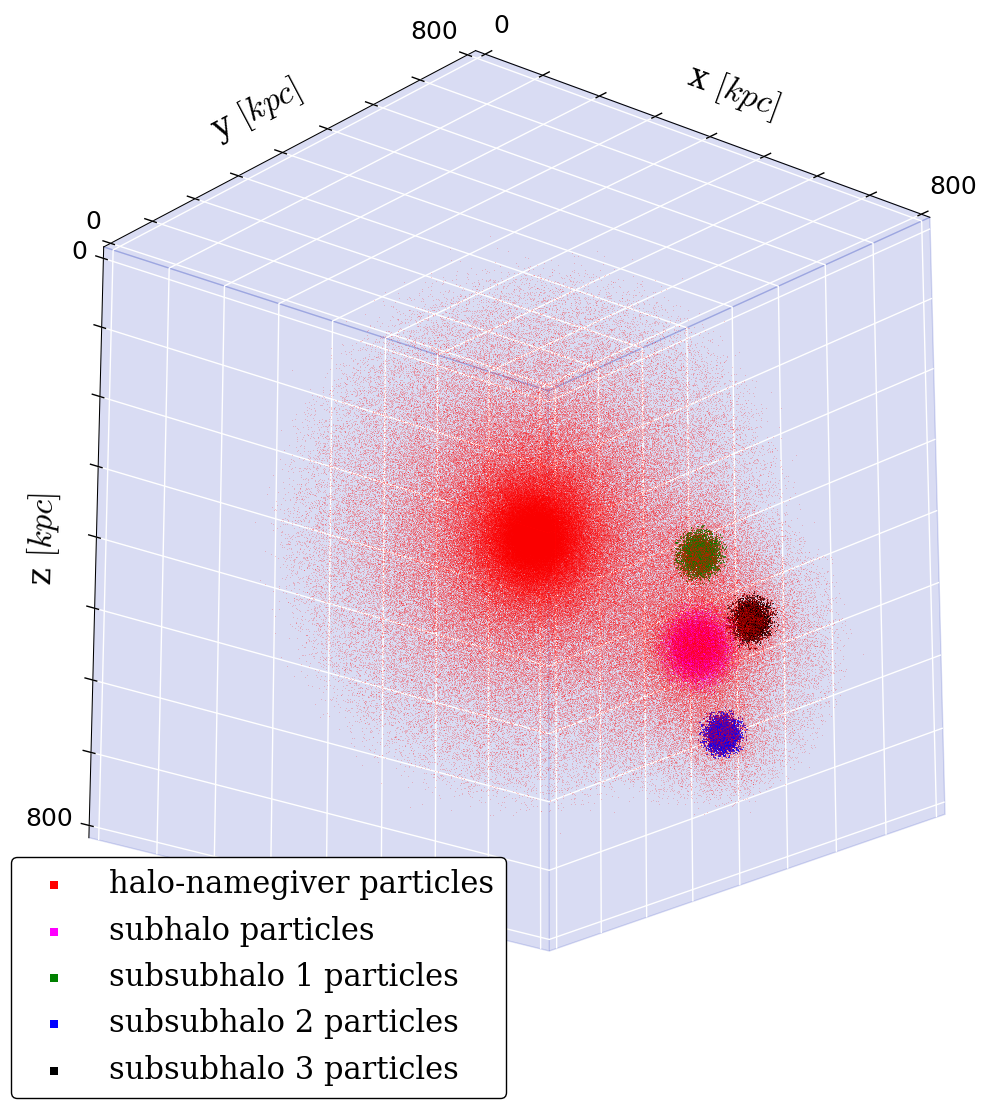
\includegraphics[width = .28\textwidth]{images/dice-sub/dice-sub-plot-halo1-iter.png}} \hspace*{-1em}&
%			{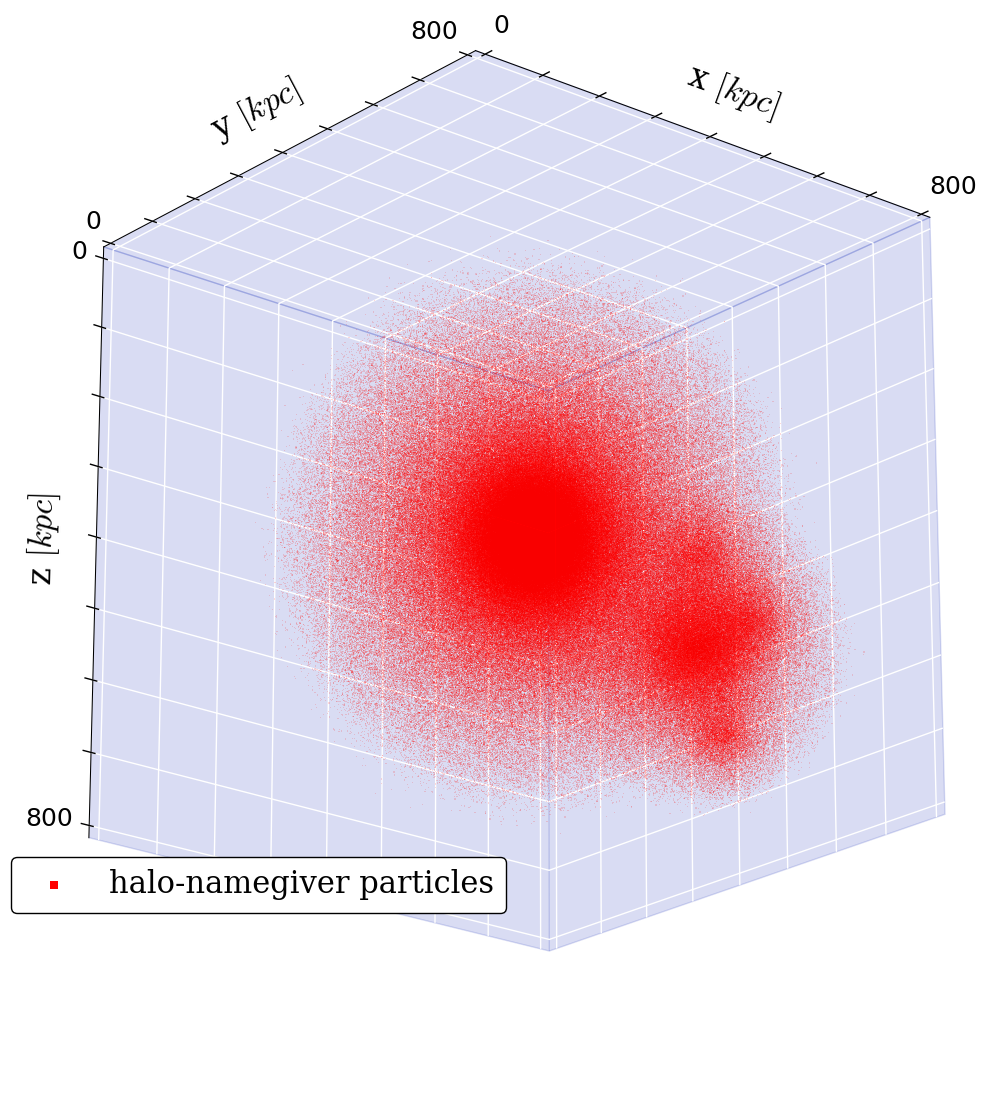
\includegraphics[width = .28\textwidth]{images/dice-sub/dice-sub-halo-only-iter.png}} \hspace*{-1em}&
%			{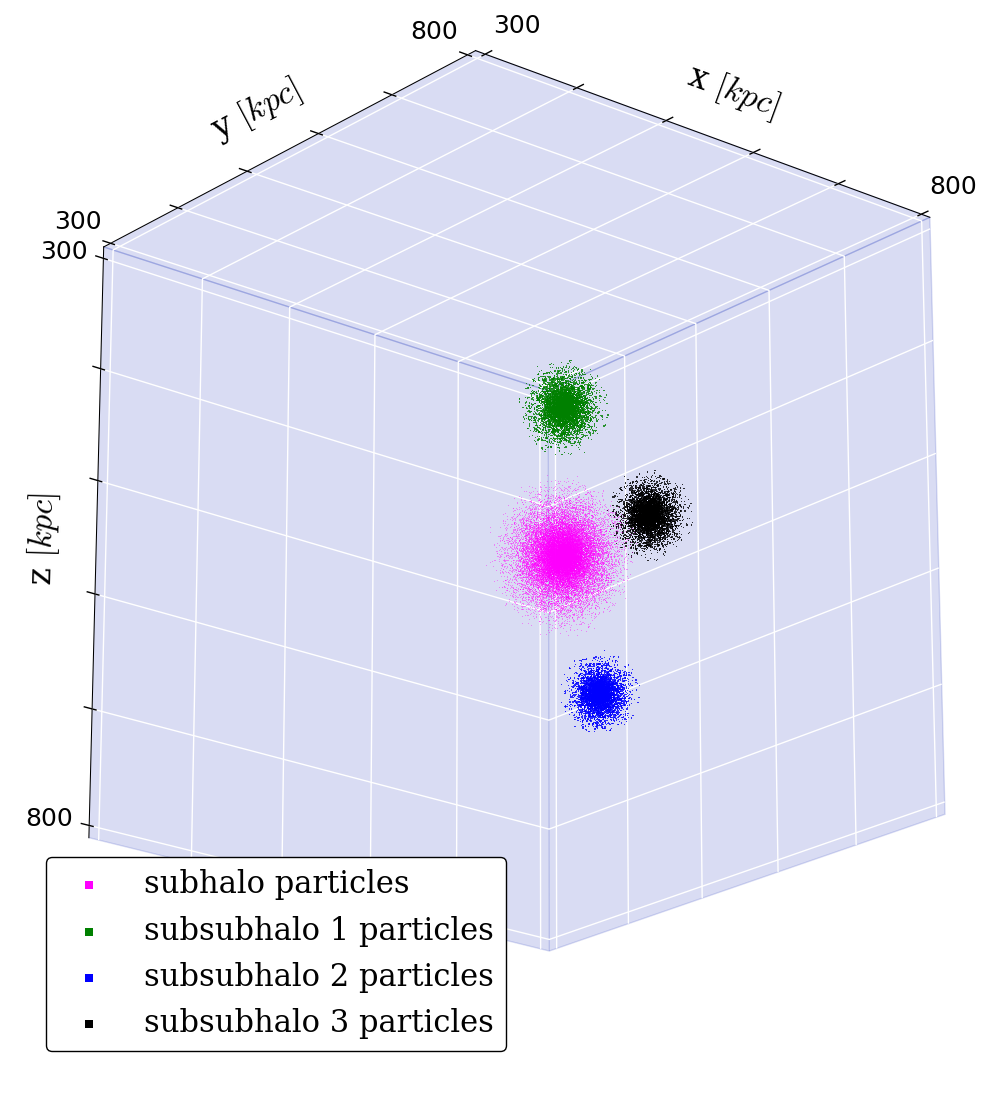
\includegraphics[width = .28\textwidth]{images/dice-sub/dice-sub-plot-subclumps-iter.png}} \\
%			%
%			%
%			\hline
%		\end{tabular}
%		\label{fig:dice_sub_results_b}
%		}
%	}
%	\caption{
%	The results of different unbinding methods on the \dt-dataset.
%	}
%	\label{fig:dice_sub_results}
%\end{sidewaysfigure}
%
%







%=====================
% Cosmo
%=====================

\begin{subfigures}
	\begin{figure}[!htbp]
		{
			\renewcommand{\arraystretch}{0.1}		
			\centering	
			%	\subfloat[]{
			\begin{tabular}{|p{.5cm} c c|}
				\hline
				&&\\[1em]
				&	\phewon\ 	& \simple \\[1.5em]
				%
				%
				\begin{sideways}{\hspace{3cm} \textbf{All particles}}\end{sideways} \hspace*{-1em}	&		 
				{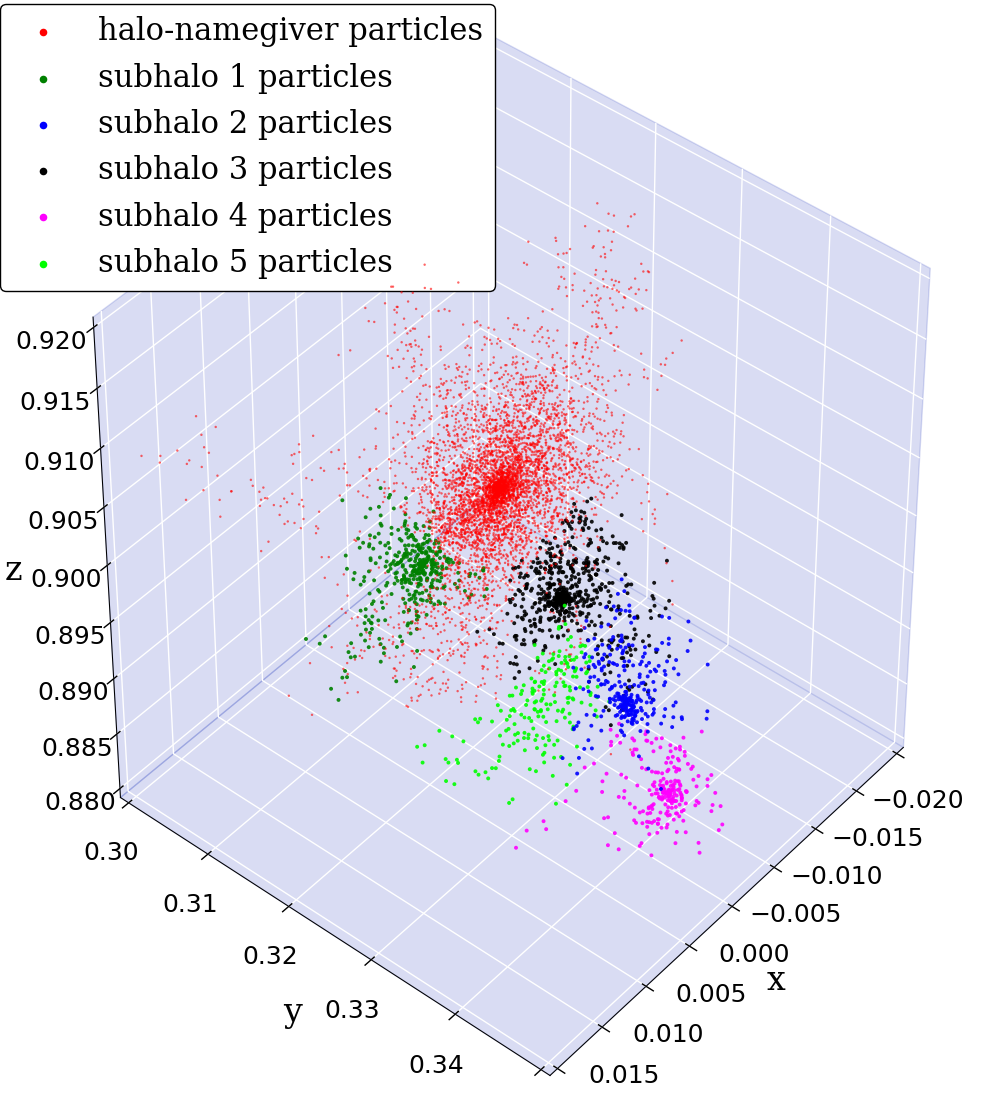
\includegraphics[width = .42\textwidth]{images/cosmo/cos-halo-66858-phew.png}} \hspace*{-1em} 	& 
				{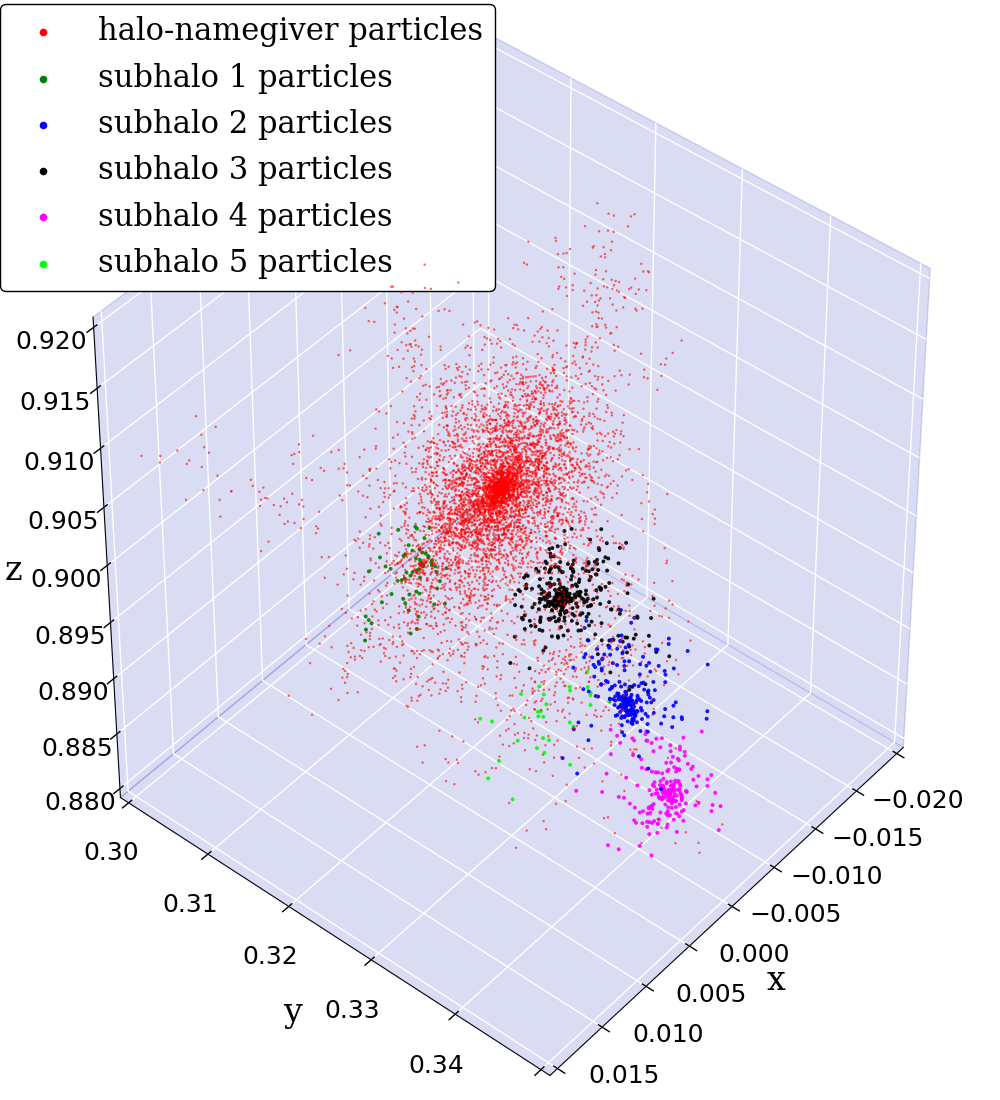
\includegraphics[width = .42\textwidth]{images/cosmo/cos-halo-66858-nosaddle.png}} \hspace*{-1em}	\\
				%
				%
				\begin{sideways}{ \hspace{.5cm}\textbf{Halo-namegiver particles only} }\end{sideways}	 \hspace*{-1em}			 &			 
				{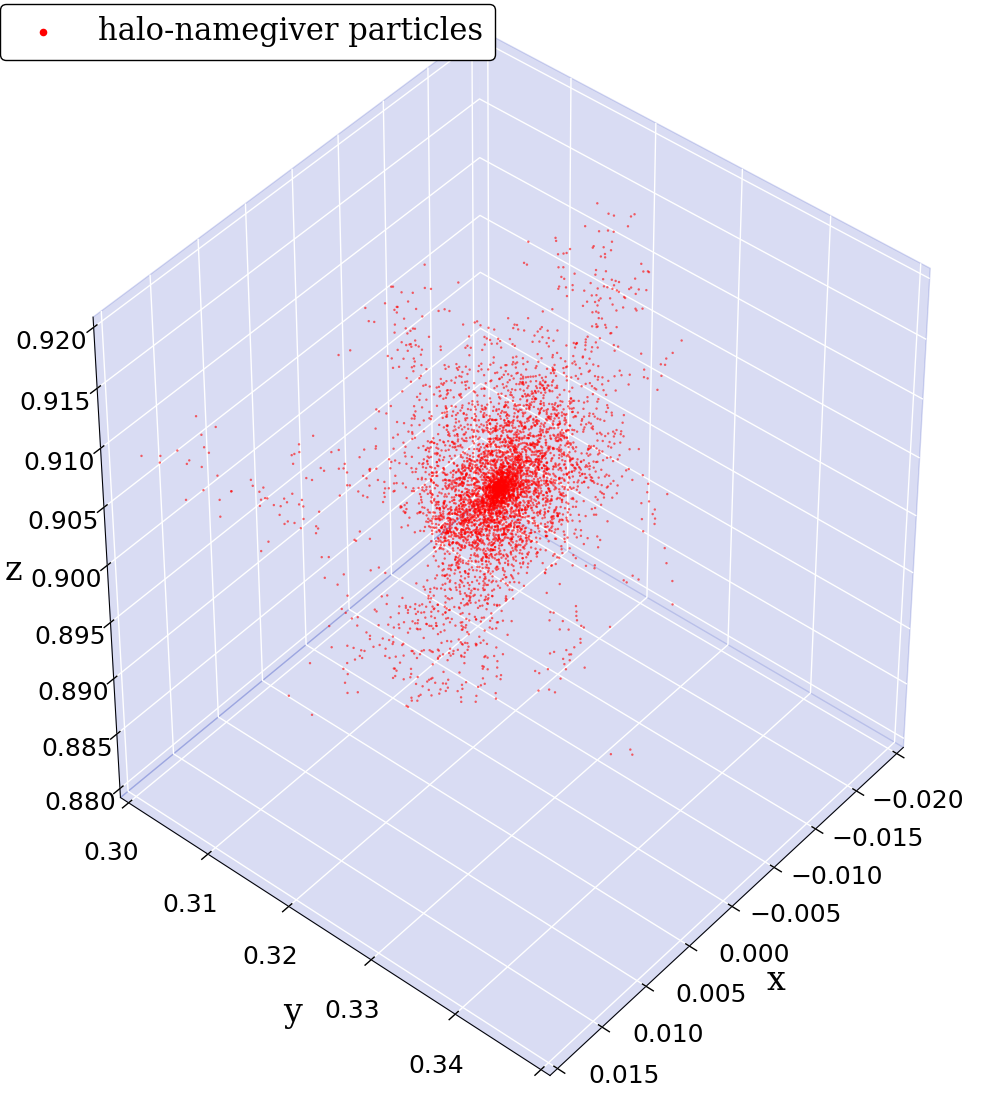
\includegraphics[width = .42\textwidth]{images/cosmo/cos-halo-66858-halo-only-phew.png}} \hspace*{-1em} 		&
				{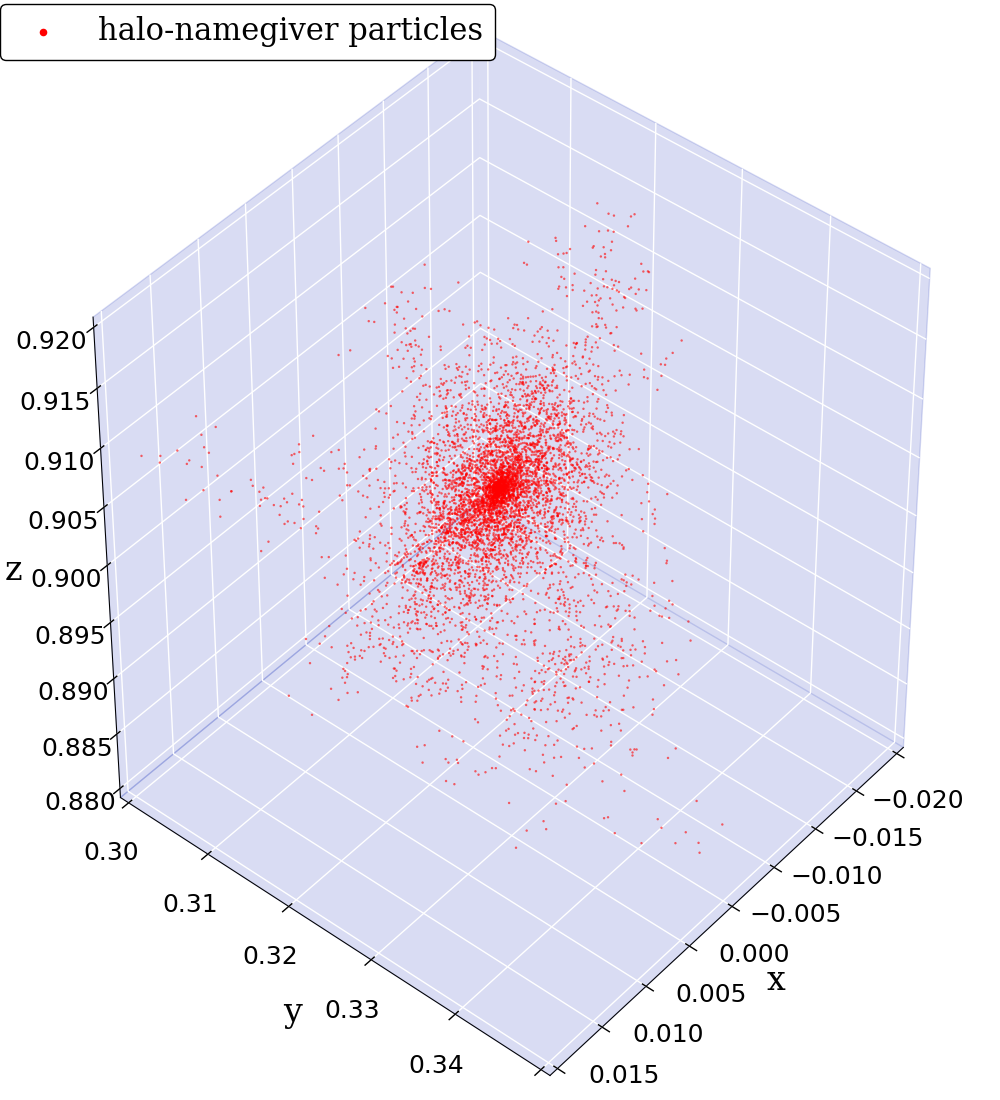
\includegraphics[width = .42\textwidth]{images/cosmo/cos-halo-66858-halo-only-nosaddle.png}} \hspace*{-1em}		\\
				%
				%
				\begin{sideways}{ \hspace{2cm}\textbf{Subhalo particles only} }\end{sideways}	 \hspace*{-1em}			 &
				{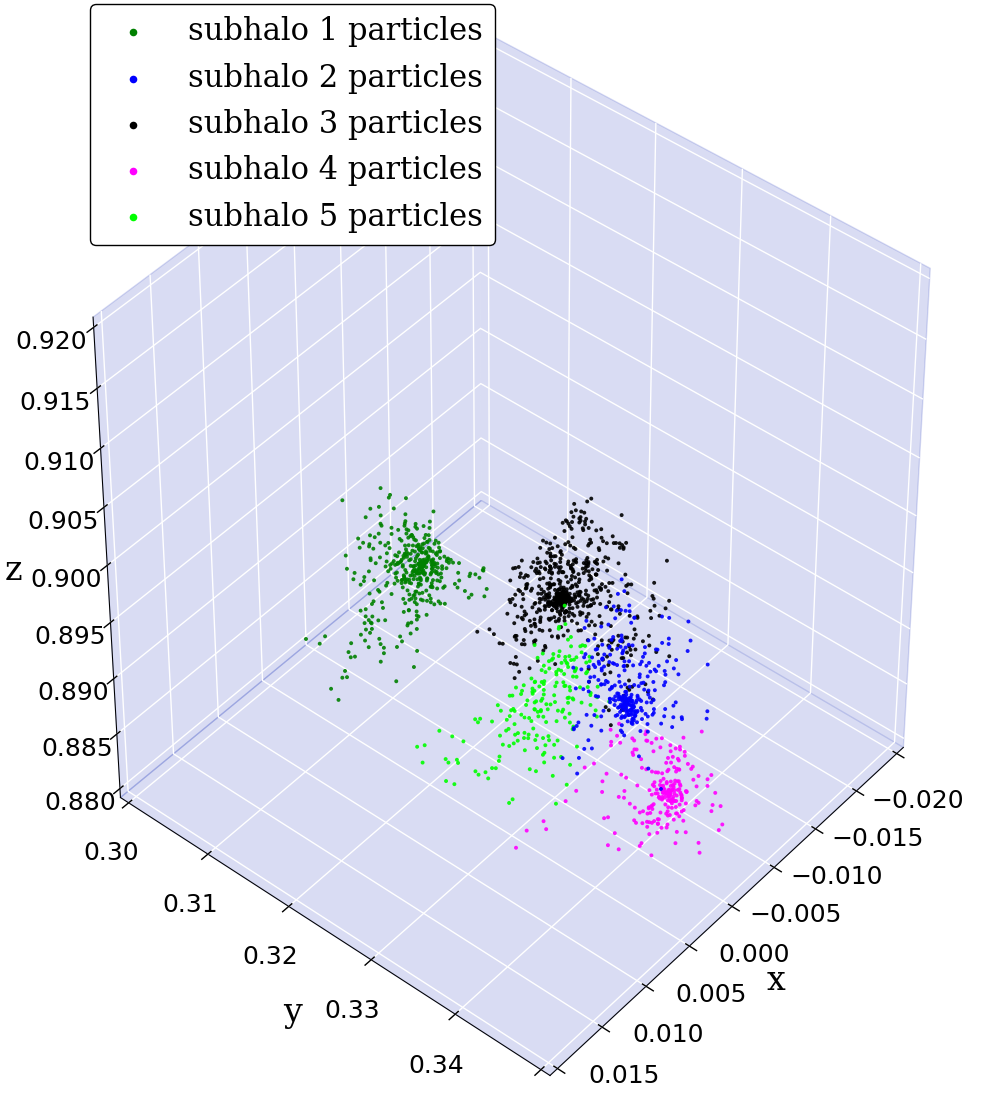
\includegraphics[width = .42\textwidth]{images/cosmo/cos-halo-66858-subhalo-only-phew.png}} &
				{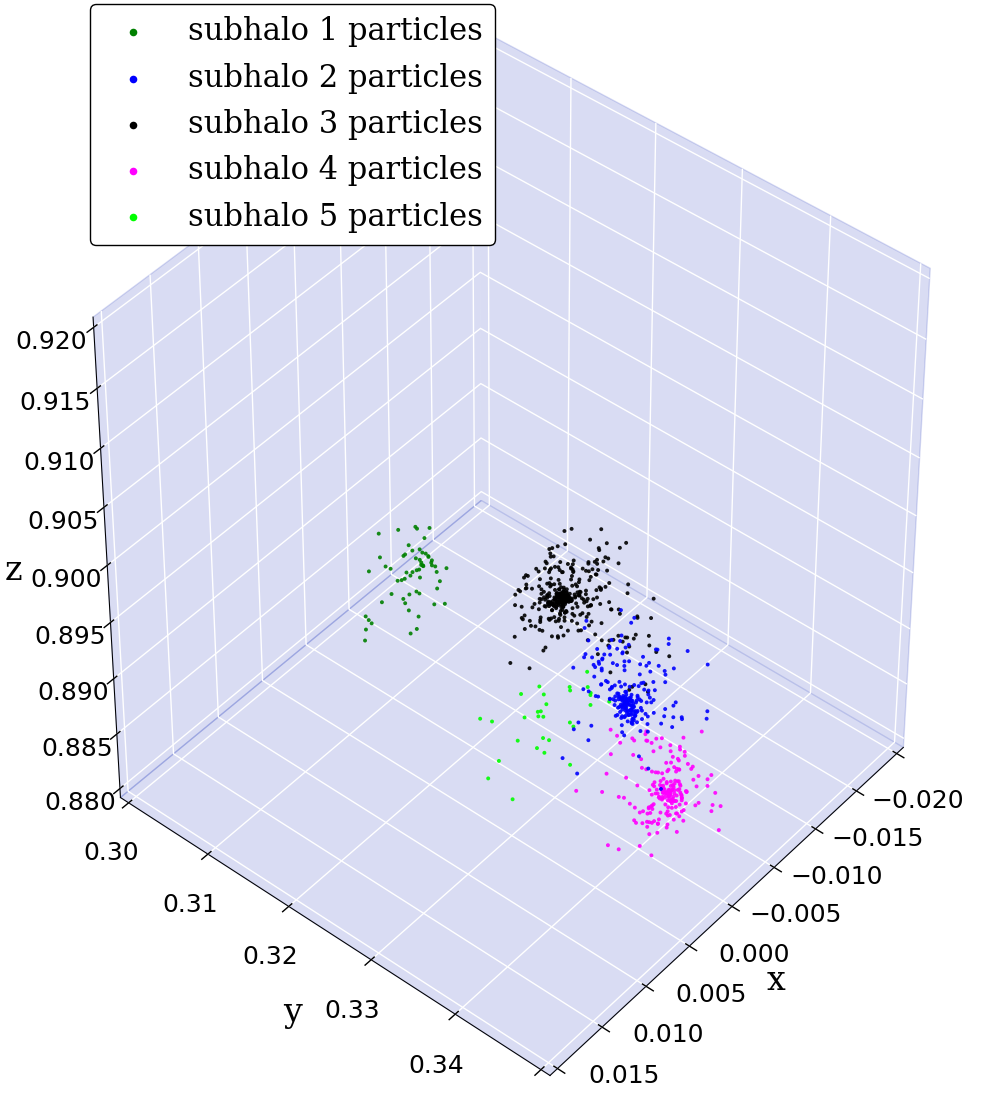
\includegraphics[width = .42\textwidth]{images/cosmo/cos-halo-66858-subhalo-only-nosaddle.png}} \\
				\hline
			\end{tabular}
			\caption{\label{fig:cosmo_results_a}The results of \phewon\ and \simple\ unbinding of the \cosmo-dataset: All particles, halo-namegiver particles only and subhalo particles only.}
		}
	\end{figure}
	%=================================================
	%=================================================
	%=================================================
	\begin{figure}[!htbp]%\ContinuedFloat
		{
			\renewcommand{\arraystretch}{0.1}
			\centering	
			\begin{tabular}{|p{.5cm} c c|}
				\hline
				&&\\[1em]
				&	\neigh\ 	& \iter \\[1.5em]
				%
				%
				\begin{sideways}{\hspace{3cm} \textbf{All particles}}\end{sideways} \hspace*{-1em}	&		 
				{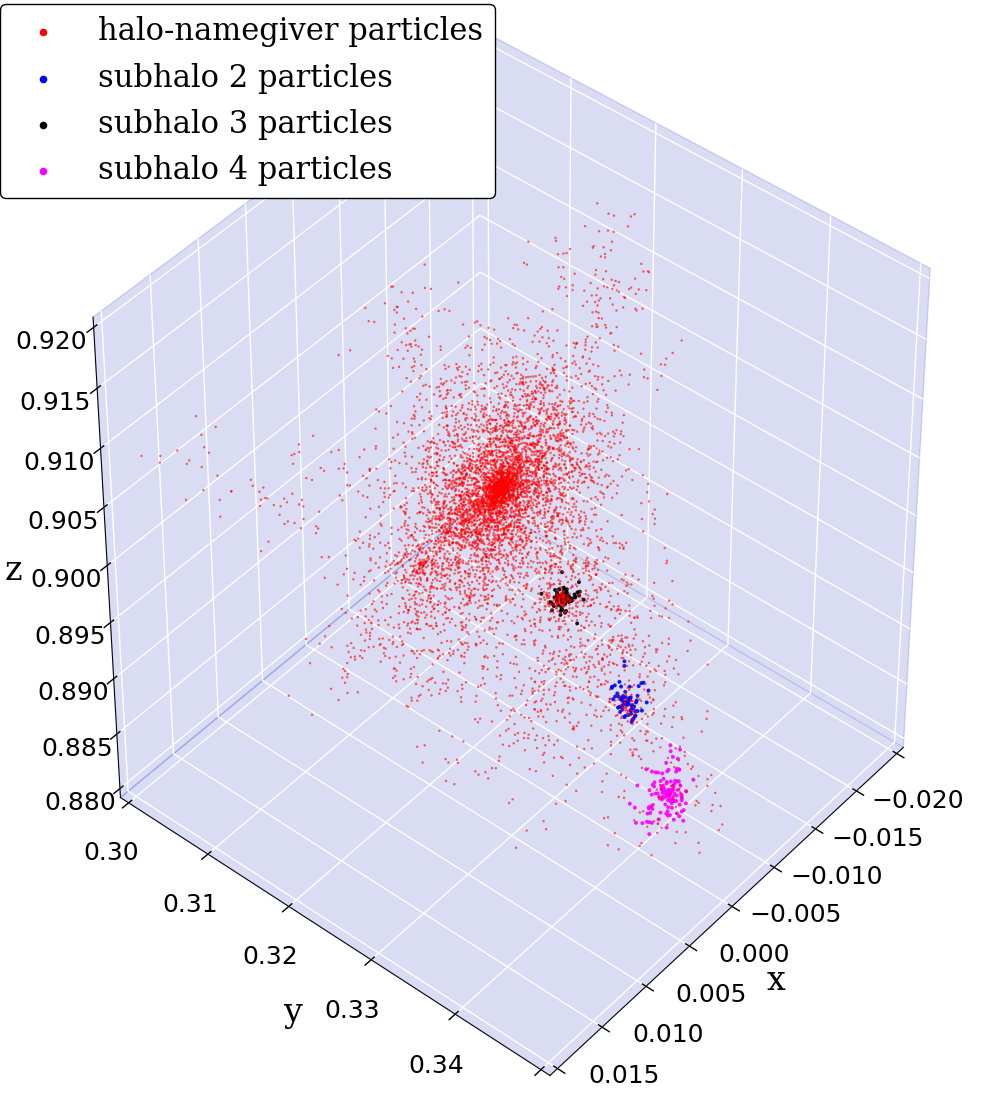
\includegraphics[width = .42\textwidth]{images/cosmo/cos-halo-66858-saddle.png}} \hspace*{-1em} 	& 
				{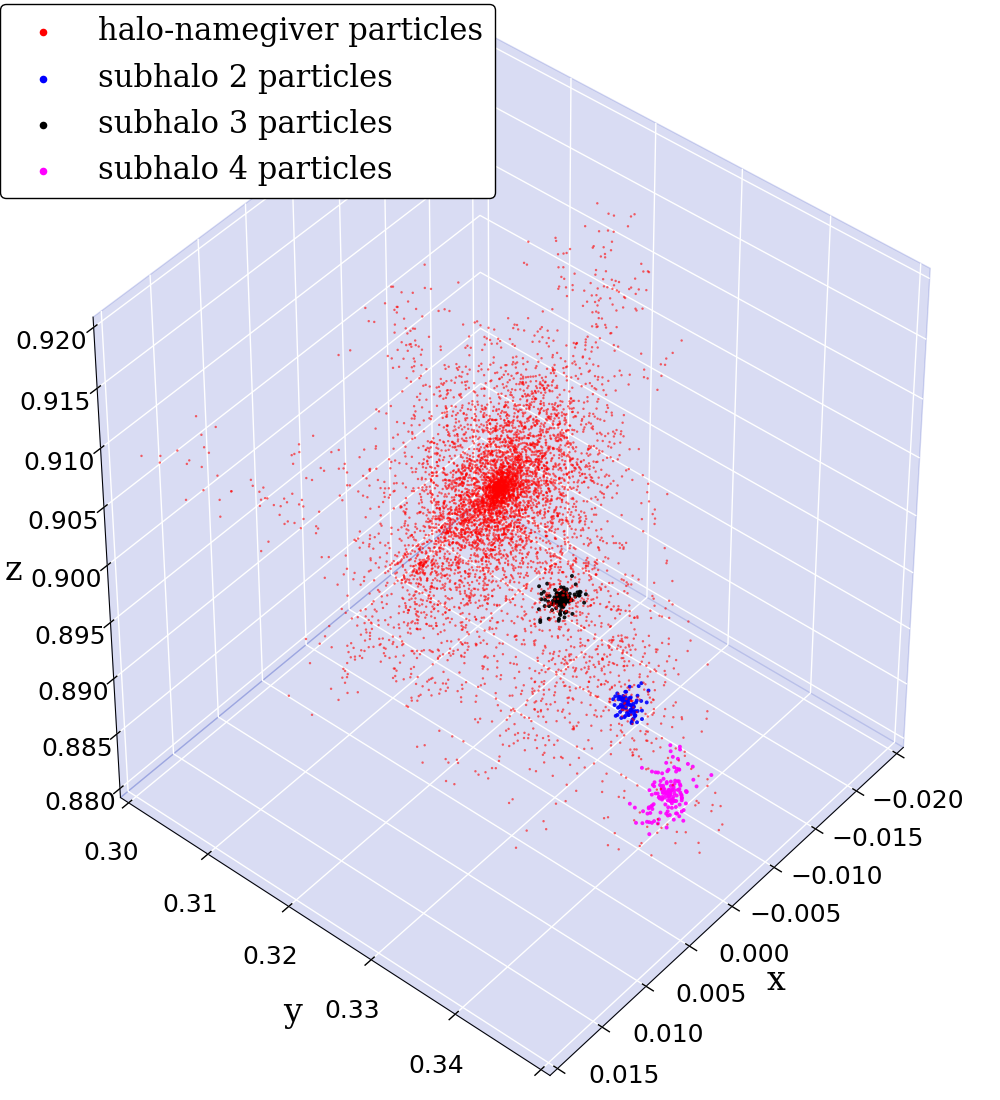
\includegraphics[width = .42\textwidth]{images/cosmo/cos-halo-66858-iter.png}} \hspace*{-1em}	\\
				%
				%
				\begin{sideways}{ \hspace{.5cm}\textbf{Halo-namegiver particles only} }\end{sideways}	 \hspace*{-1em}			 &			 
				{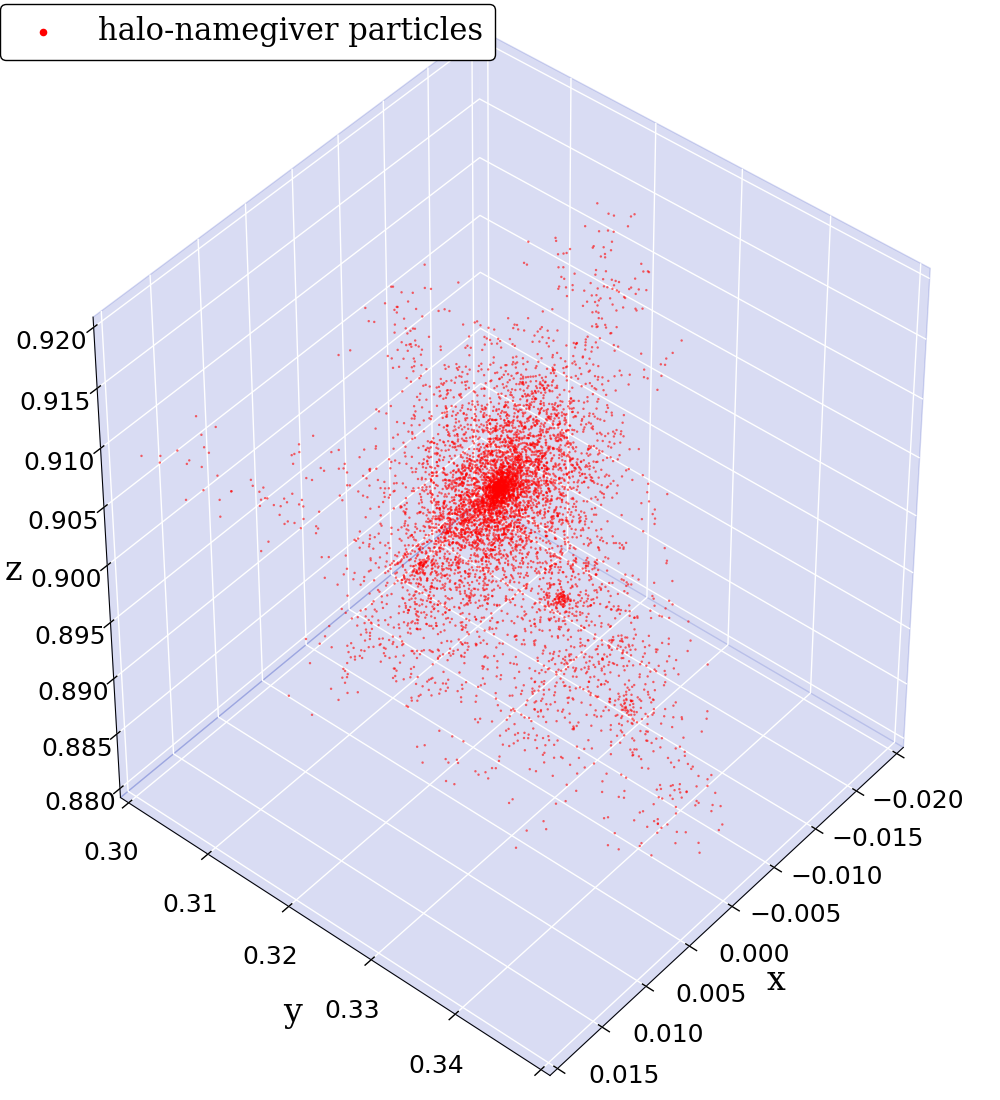
\includegraphics[width = .42\textwidth]{images/cosmo/cos-halo-66858-halo-only-saddle.png}} \hspace*{-1em} 		&
				{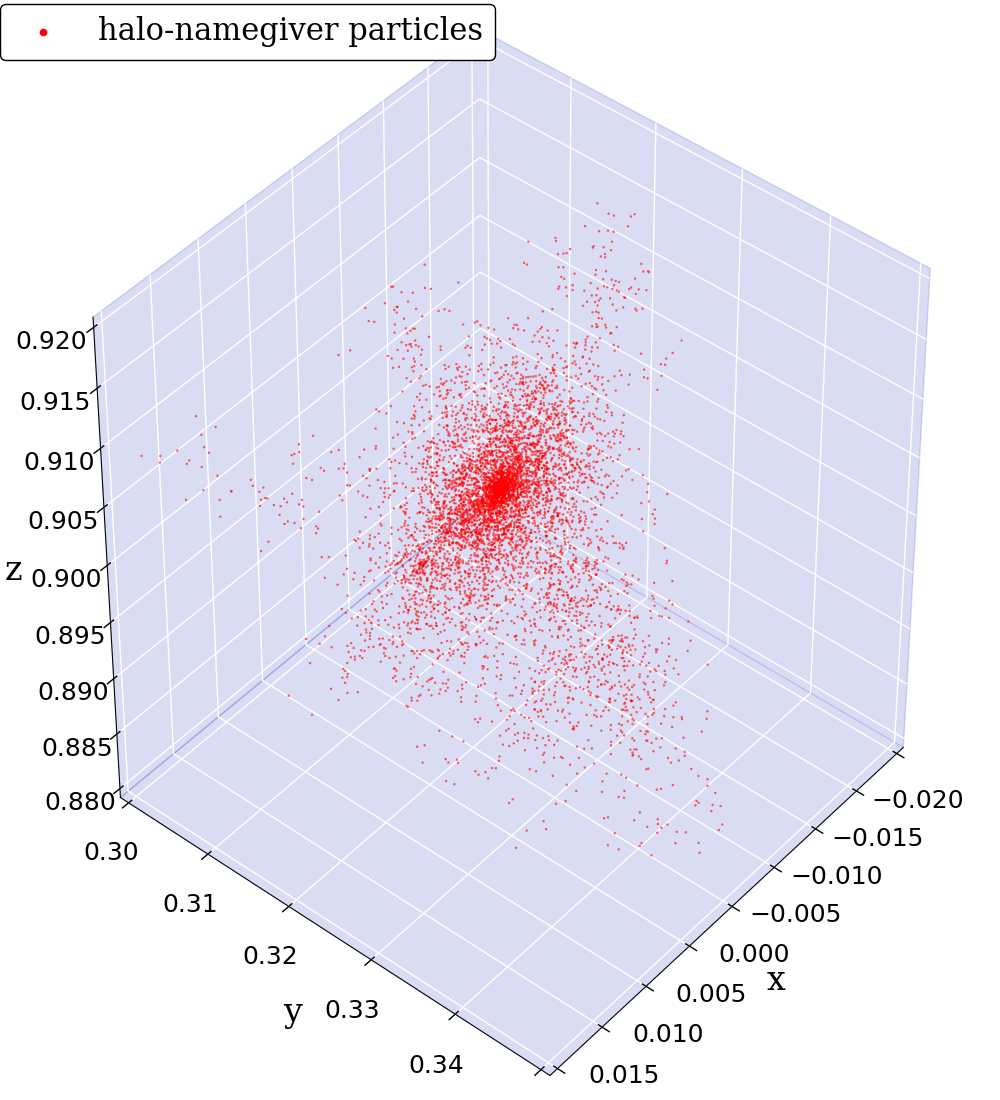
\includegraphics[width = .42\textwidth]{images/cosmo/cos-halo-66858-halo-only-iter.png}} \hspace*{-1em}		\\
				%
				%
				\begin{sideways}{ \hspace{2cm}\textbf{Subhalo particles only} }\end{sideways}	 \hspace*{-1em}			 &
				{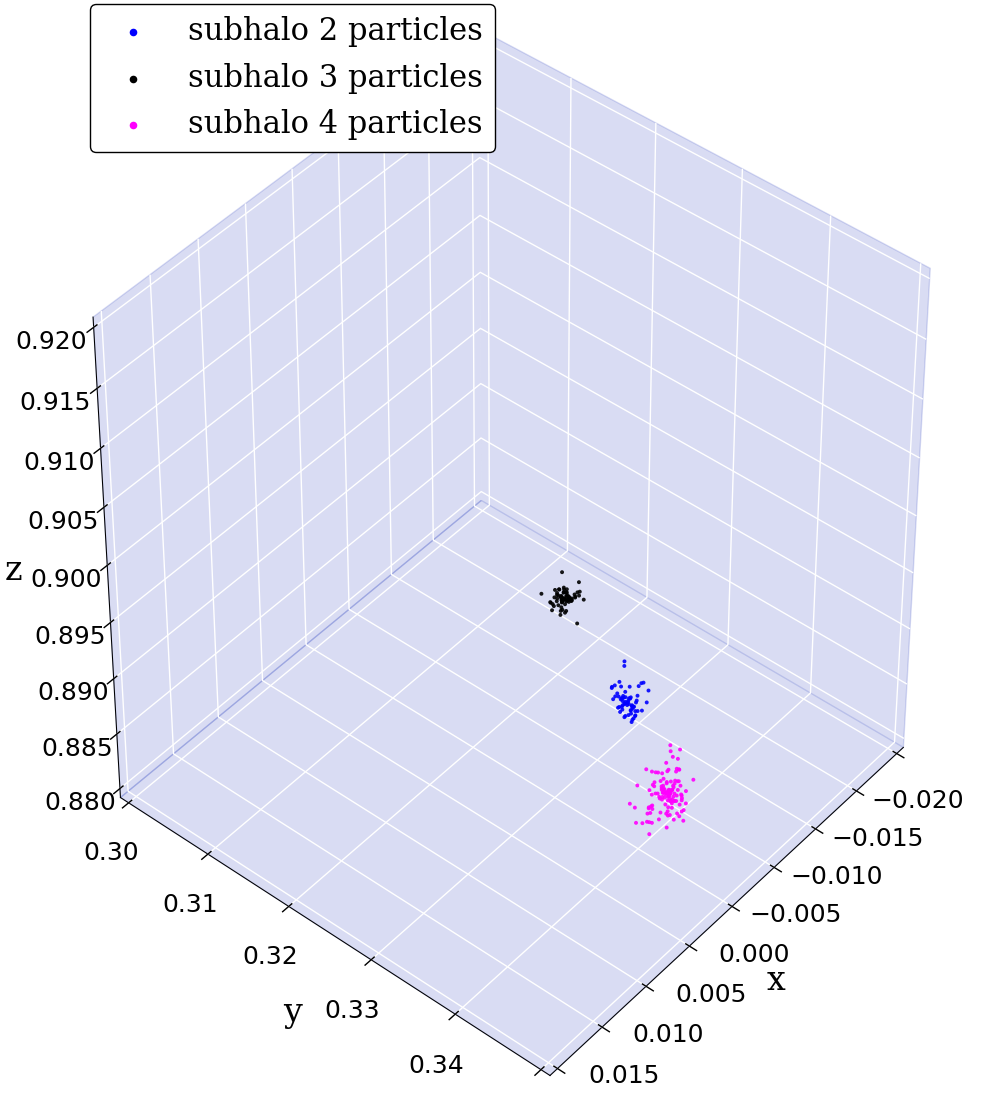
\includegraphics[width = .42\textwidth]{images/cosmo/cos-halo-66858-subhalo-only-saddle.png}} &
				{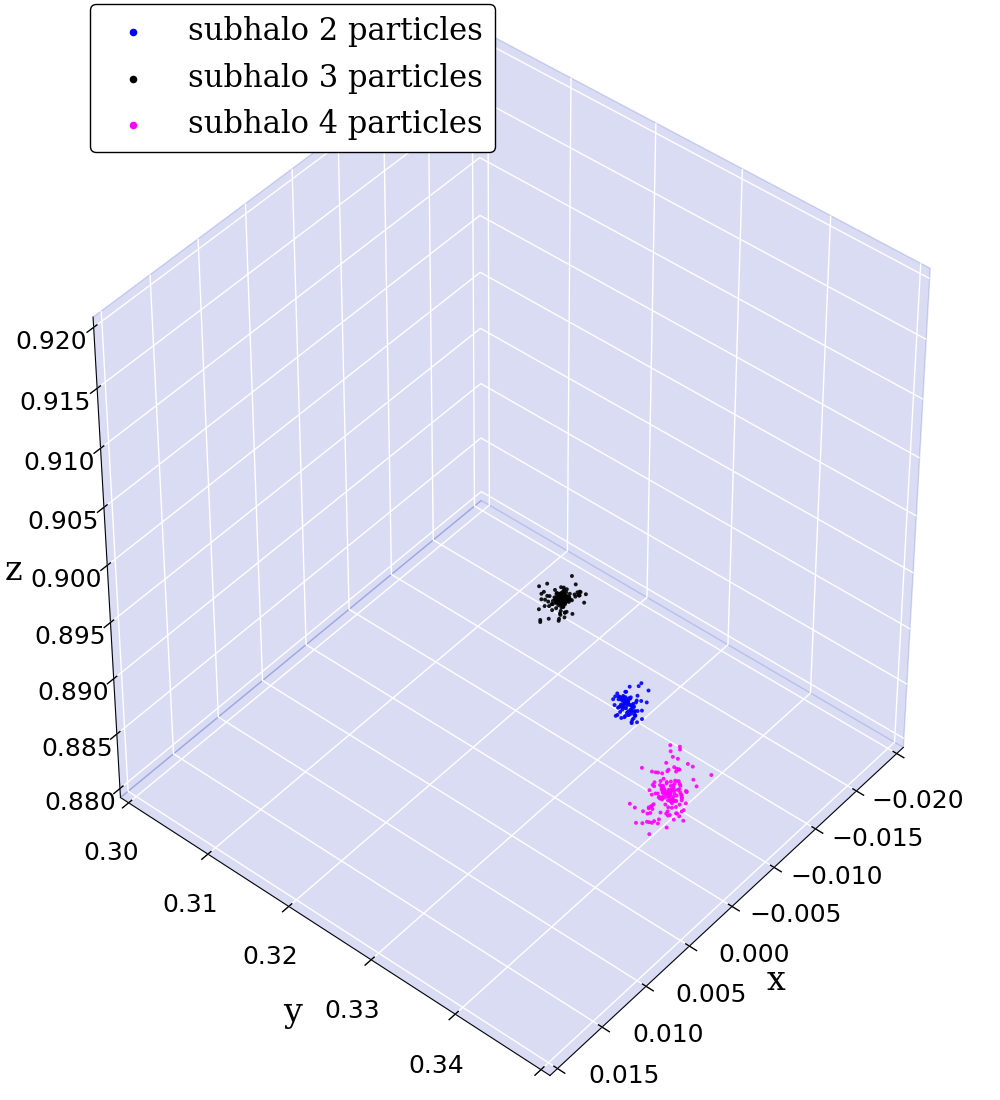
\includegraphics[width = .42\textwidth]{images/cosmo/cos-halo-66858-subhalo-only-iter.png}} \\
				\hline
			\end{tabular}
			\caption{\label{fig:cosmo_results_b}
				The results of \neigh\ and \iter\ unbinding of the \cosmo-dataset: All particles, halo-namegiver particles only and subhalo particles only.
			}
		}
	\end{figure}
	\label{fig:cosmo_results}
\end{subfigures}






































%
%
%\begin{sidewaysfigure}[!htbp]
%	{\renewcommand{\arraystretch}{0.1}
%		
%	\subfloat[The results of \phewon\ and \simple\ unbinding of the \cosmo-dataset: All particles, halo-namegiver particles only and subhalo particles only.]{
%		\begin{tabular}{|p{1cm} c c c|}
%			\hline
%			&&&\\[1em]
%													&
%			\textbf{All particles} 					&
%			\textbf{Halo-namegiver particles only} 	&
%			\textbf{Subhalo particles only} 		\\[1em]
%			%
%			%
%			\begin{sideways}{\hspace{3cm} \phewon}\end{sideways} \hspace*{-1em}%		 
%			& {\includegraphics[width = .42\textwidth]{images/cosmo/cos-halo-66858-phew.png}} \hspace*{-1em}%
%			& {\includegraphics[width = .42\textwidth]{images/cosmo/cos-halo-66858-halo-only-phew.png}} \hspace*{-1em}% 
%			& {\includegraphics[width = .42\textwidth]{images/cosmo/cos-halo-66858-subhalo-only-phew.png}} \\
%			%
%			%
%			\begin{sideways}{ \hspace{3cm}\simple\ unbinding }\end{sideways}	 \hspace*{-1em}			 &
%			{\includegraphics[width = .42\textwidth]{images/cosmo/cos-halo-66858-nosaddle.png}} \hspace*{-1em}&
%			{\includegraphics[width = .42\textwidth]{images/cosmo/cos-halo-66858-halo-only-nosaddle.png}} \hspace*{-1em}&
%			{\includegraphics[width = .42\textwidth]{images/cosmo/cos-halo-66858-subhalo-only-nosaddle.png}} \\
%			\hline
%		\end{tabular}
%		\label{fig:cosmo_results_a}
%		}
%	}
%	\phantomcaption
%\end{sidewaysfigure}
%%=================================================
%%=================================================
%%=================================================
%\begin{sidewaysfigure}[!htbp]\ContinuedFloat
%	\footnotesize
%	{\renewcommand{\arraystretch}{0.1}
%	\subfloat[The results of \neigh\ and \iter\ unbinding of the \cosmo-dataset: All particles, halo-namegiver particles only and subhalo particles only.]{
%		\begin{tabular}{|p{1cm} c c c|}
%			\hline
%			&&&\\[1em]
%													&
%			\textbf{All particles} 					&
%			\textbf{Halo-namegiver particles only} 	&
%			\textbf{Subhalo particles only}			\\[1em]
%			%
%			%
%			\begin{sideways}{ \hspace{3cm}\neigh\ unbinding }\end{sideways}		\hspace*{-1em}		 &		
%			{\includegraphics[width = .42\textwidth]{images/cosmo/cos-halo-66858-saddle.png}}\hspace*{-1em} &
%			{\includegraphics[width = .42\textwidth]{images/cosmo/cos-halo-66858-halo-only-saddle.png}}\hspace*{-1em} &
%			{\includegraphics[width = .42\textwidth]{images/cosmo/cos-halo-66858-subhalo-only-saddle.png}} \\
%	%		%
%	%		%
%			\begin{sideways}{\hspace{3cm} \iter\ unbinding }\end{sideways}		\hspace*{-1em}		 &		
%			{\includegraphics[width = .42\textwidth]{images/cosmo/cos-halo-66858-iter.png}} \hspace*{-1em}&
%			{\includegraphics[width = .42\textwidth]{images/cosmo/cos-halo-66858-halo-only-iter.png}} \hspace*{-1em}&
%			{\includegraphics[width = .42\textwidth]{images/cosmo/cos-halo-66858-subhalo-only-iter.png}} \\
%			%
%			%
%			\hline
%		\end{tabular}
%		\label{fig:cosmo_results_b}
%		}
%	}
%	\caption{
%	The results of different unbinding methods on the \cosmo-dataset.
%	}
%	\label{fig:cosmo_results}
%\end{sidewaysfigure}
































%=====================
% Resource Usage
%=====================

\subsection{Resource usage}

\begin{table}[!htb]
	{\footnotesize
	\begin{centering}
		\def\arraystretch{1.2}
		\begin{tabular}[t]{l | R{1.7cm} |  R{1.7cm} |  R{1.8cm}  ||  R{1.7cm}  |  R{1.7cm}  |  R{1.8cm}  |}
			%
			%=======================
			% DICE TWO 
			%=======================
			%
			\cline{2-7}
							& \multicolumn{6}{|c|}{\textbf{\dt-dataset} ($2.4 \cdot 10^5$ particles, 21.8$\%$ of which are in subhalos) } \\
			\cline{2-7}
							& \multicolumn{3}{|c||}{Sequential execution} & \multicolumn{3}{c|}{Parallel execution} \\
			\cline{2-7}
							&\ramses\	 & \phew    &  unbinding & \ramses  & \phew\      &  unbinding\\
			\hline
%			Wall time (s)	&	16.19    &	19.85  	 &	21.82	 &	 6.52	  & 	8.93  	 &	12.08	\\[-1.5ex]
%							& +34.8 $\%$ & +9.9 $\%$ &	-		 & +85.3 $\%$ & +35.3 $\%$   &	-		\\[1.5ex]
			CPU time (s)	&	16.18	 &	19.83	 &	21.81	 &	26.06	  &	35.71		 &	48.30	\\[-1.5ex]
							& +34.8 $\%$ & +10.0 $\%$& -		 & +85.3 $\%$ & +35.3 $\%$   &  -		  \\[1.5ex]
			PMUPC (Mb)		&	390.50	 &	401.37	 &	452.37	 &	396.76	  &	551.09	     &	572.54	\\[-1ex]
							& +15.8 $\%$ & +12.7 $\%$& -		 & +44.3 $\%$ & +3.9 $\%$    &  -		\\
			\hline
			\multicolumn{7}{c}{}\\
			%
			%=======================
			% DICE SUB 
			%=======================
			%
			\cline{2-7}
							& \multicolumn{6}{|c|}{\textbf{\ds-dataset} ($1.26 \cdot 10^6$ particles, 23.4$\%$ of which are in subhalos) } \\
			\cline{2-7}
							& \multicolumn{3}{|c||}{Sequential execution} & \multicolumn{3}{c|}{Parallel execution} \\
			\cline{2-7}
							&\ramses\	 & \phew    &  unbinding & \ramses\ & \phew\      &  unbinding \\
			\hline
%			Wall time (s)	&	56.77	 &	82.32	 &	88.41	 &	70.40	  &	 90.33	     &	111.24	\\[-1.5ex]
%							& +55.7 $\%$ & +7.4 $\%$ &  -		 &+58.0 $\%$  & +23.1 $\%$   &  -   \\[1.5ex]
			CPU time (s)	&	56.77	 &	82.31	 &	88.41	 &	281.60	  &	361.30		 &	444.93	\\[-1.5ex]
							& +55.7 $\%$ & +7.4 $\%$ &	-		 &+58.0 $\%$  &	+23.1 $\%$   &	- 	\\[1.5ex]
			PMUPC (Mb)		&	1313.36	 &	1358.45	 &	1562.06	 &	405.96	  &	565.26		 &	625.64	\\[-1ex]
							& +18.9 $\%$ & +15.0 $\%$&   -		 & +54.1 $\%$ &+10.7 $\%$    &   -		\\
			\hline
			\multicolumn{7}{c}{}\\
			%
			%=======================
			% COSMO 
			%=======================
			%
			\cline{2-7}
							& \multicolumn{6}{|c|}{\textbf{\cosmo-dataset} ($128^{3}$ particles, 9.0$\%$ of which are in subhalos) } \\
			\cline{2-7}
							& \multicolumn{3}{|c||}{Sequential execution} & \multicolumn{3}{c|}{Parallel execution} \\
			\cline{2-7}
							& \ramses	& \phew    &  unbinding & \ramses\ & \phew      &  unbinding\\
			\hline
%			Wall time (s)	&	-		&	-		&	-		&	95.94	 &	108.24	    &	112.12	\\[-1.5ex]
%							&			&			&			& +16.9 $\%$ & +3.6 $\%$    & -			\\[1.5ex]
			CPU time (s)	&	-		&	-		&	-		&	383.72	 &	432.93	  	&	448.46	\\[-1.5ex]
							&   		&			&			& +16.9 $\%$ & +3.6 $\%$    & -			\\[1.5ex]
			PMUPC (Mb)		&	-		&	-		&	-		&	1335.61	 &	1342.77		&	1526.65	\\[-1ex]
							&			&			&			& +14.3 $\%$ & +13.7 $\%$   &	-		\\
			\hline
			\multicolumn{7}{c}{}
		\end{tabular}
	\end{centering}
	} %footnotesize
	\caption{%
		Performance measurements for sequential and parallel executions on the three datasets used for tests. 
		The parallel runs were executed on 4 cores. The CPU time of the parallel executions is the total CPU time of all 4 cores. ``\emph{PMUPC}'' stands for ``peak memory usage per core''.		
		``\ramses'' measurements consist of advancing the simulation for a timestep. ``\phew'' runs do the same, but include clump finding, while ``unbinding'' runs include clump finding and particle unbinding.
		The given values are the highest values out of 10 measurements. 
		The percentages below the measurements give the relative additional cost of the unbinding run.
	}%
	\label{tab:resource-usage-measurements}%
\end{table}


It was not possible to measure the resource usage of the unbinding algorithm in isolation, because it only works within the frame of \ramses\ and \phew. 
That is why the CPU time and the peak memory consumption per core (PMCPC) were measured not only with the unbinding procedure executed (``unbinding runs''), but also when the clump finding was performed without unbinding (``\phew\ runs'') and runs without clump finding at all (``\ramses\ runs'').
Each run consist of advancing the simulation for one time step.
The clump finding and unbinding procedures, when used in a run, are always called twice: First after the initialisation, then after the advance in time of the simulation.

The measurements were made using the GNU \verb|time| version 1.7 command on an Intel Core i7-6700HQ processor with four cores.
For the two datasets created with \dice, both sequential runs, performed on only one core, as well as parallel runs, performed on four cores (without hyper-threading) were measured.
Measurements of sequential runs of the \cosmo-dataset were not possible, because of the lack of a dataset that can be run on only one core.
The ``unbinding runs'' are set up identically to \iter-runs because this method requires the most resources.
100 mass bins and iterative clump properties determination with a convergence limit $\varepsilon$ of 0.01 were used.
Each run was repeated ten times, out of which the highest resource usage is shown in table \ref{tab:resource-usage-measurements}.

These measurements are mostly meant as a guideline for future users.
Very little comparisons can be made between the three datasets, because the necessary resources depend on a multitude of factors, such as particle numbers, how far the mesh will be refined, the number of particles that will end up being in halos and subhalos and so forth, some of which are very difficult to control.

The additional computational cost is expected to be strongly affected by the number of particles that are in subhalos, as these are the ones that the unbinding procedure works on. 
Particles in halos are not considered for unbinding.
Comparing the CPU times of the \ds-dataset with the times of the \cosmo-dataset supports this expectation.
Even though the \cosmo-dataset contains $\sim 1.7$ as many total particles as the \ds-dataset, it has $\sim 1.6$ times less particles that are actually in subhalos.
If the number of particles in subhalos wasn't an important factor for the computational cost, the CPU times of the runs including the unbinding procedure shouldn't be nearly identical.

The measurements also indicate that the relative additional cost compared to the runs without unbinding decreases with increasing total particle number.
This may be explained by the fact that most particles that are found to be in a structure will be in halos, thus won't contribute significantly to the cost of the unbinding procedure, while raising the expenses for \ramses\ and \phew.
This interpretation is supported in the case of the two datasets created by \dice, where the \ds-dataset contains more particles in subhalos both in absolute number and percentage, but requires noticeably less relative additional resources.

The additional required resources seem acceptable for a code designed to work on-the-fly, particularly so in the case of the \cosmo-dataset. 
If required, the execution time might be accelerated by vectorising the code, which for most parts hasn't been done yet.




